\section{Аналіз та вибір навігаційного забезпечення}

Відповідно до розробленої у НДР „”( \textbf{[TODO добавить номер НДР]}) методики 
побудови комплексної навігаційної системи, задача створення 
інерціально-супутникової системи навігації для визначення координат 
місцеположення рухомого об'єкта, передбачає:

Обґрунтування, та вибір (або розробка) структури і варіанту комплексування 
інтегрованої інерціально-супутникової системи на основі аналізу класу і 
технічних характеристик ЛА, з урахуванням діапазонів кутів крену та тангажа, 
ударних навантажень, максимальних швидкостей та прискорень, орієнтуючись на 
тип точності основних навігаційних засобів (комплекс середньої точності, 
низької вартості та малих габаритів і маси), масогабаритні характеристики, 
споживану потужність та вартість обладнання. 

Формулювання основних характеристик комплексної системи у вигляді граничних 
погрішностей навігаційних визначень;

Для обраного варіанту інтегрованої інерціально-супутникової системи 
обирається з представленого на ринку модельного ряду авіаційних 
прийомоіндикаторів супутникових систем потрібний за технічними 
характеристиками та розв'язуваними задачами тип прийомоіндикатора, або 
формулюються технічні вимоги  на розробку такого прийомоіндикатора. 

Для обраного варіанту інерціально-супутникової системи обирається схема 
інерціальної навігаційної системи;

На основі аналізу варіантів побудови датчиків первісної інформації БІНС
\nomenclature{БІНС}{безплатформенна інерціальна навігаційна система} 
і основних характеристик інерціальных датчиків, використовуючи методику 
попереднього оцінювання точностних характеристик ДПІ 
\nomenclature{ДПІ}{датчики первинної інформації}   
БІНС, обираються типи датчиків первісної інформації БІНС;

Ґрунтуючись на аналізі типових польотних завдань, що виконує даний клас ЛА
\nomenclature{ЛА}{літальний апарат}    
або БПЛА, обираються варіанти систем координат, в яких повинні формулюватися 
кінематичні рівняння алгоритмів БІНС;

Для обраних варіантів систем координат розробляються кінематичні рівняння 
алгоритмів БІНС, в яких при завданні орієнтацію зв'язаної системи координат 
відносно опорної за рішенням проектанта можуть бути використані алгоритми 
із застосуванням направляючих косинусів, кутів Ейлера, компонентів векторів 
кінцевого повороту й орієнтації, параметрів Родріга-Гамільтона, параметрів 
Келі-Клєйна;

Після прийняття рішення про корекцію вертикального каналу інтегрованої 
інерціально-супутникової системи від вимірника барометричної висоти обирається 
тип баровисотоміра, або формулюються технічні вимоги на розробку такого 
вимірника, обирається тип датчика статичного тиску, розробляються алгоритми 
обчислення барометричної висоти за інформацією від датчика статичного тиску;

Випереджаючи розробку алгоритмів комплексної обробки навігаційної 
інформації, виконується розробка математичних моделей похибок датчиків, 
БІНС, СНС та вимірника барометричної висоти. Причому, якщо за моделі 
похибок датчиків БІНС, СНС та вимірника барометричної висоти можна 
застосовувати відомі математичні моделі, то математичну модель похибок 
БІНС потрібно формулювати базуючись на розроблених алгоритмах ідеальної 
роботи БІНС;

Після прийняття рішення про застосування в інтегрованої інерціально-супутникової 
системі оптимальної схеми комплексування виконується розробка алгоритмів 
комплексної обробки навігаційної інформації від БІНС, СНС та вимірника 
барометричної висоти на базі процедур оптимальної дискретної калманівської 
фільтрації залежно від обраного варіанту схем інтегрування: для слабкозвязаної 
або сильнозвязаної системи, з метою оцінювання похибок і введення поправок у 
вихідні дані БІНС.

\subsection{Аналіз та вибір структури та варіанту комплексування інегрованої
інерціально-супутникової системи}

Комплексна вторинна обробка інформації дає значний позитивний ефект тоді, 
коли відповідні вимірники працездатні, тобто на виходах радіонавігаційних 
вимірників, зокрема на виході корелятора приймача СНС,  є досить "хороші" 
(природно що, і в таких випадках  існують похибки слідкування) сигнали, 
сформовані в результаті первинної обробки інформації. Реальні умови застосування 
апаратури навігаційних споживачів показують, що багато вимірників, і, насамперед, 
радіотехнічні супутникові системи навігації, далеко не завжди знаходяться в 
працездатному стані. У реальних умовах нерідко спостерігається зрив супроводу 
сигналів супутників, зокрема, через багатопроменевість і дію інших завад, 
захоплення похибкових сигналів і т.п.

В теперішній час розроблені схеми можливого комплексування СНС і ІНС у чотирьох 
основних варіантах:
\begin{enumerate}
\item роздільна схема;
\item слабко зв'язана схема;
\item жорстко зв'язана схема;
\item глибоко інтегрована схема.
\end{enumerate}

Тут і в подальшому під СНС мається на увазі інтегрована СНС ГЛОНАСС/GPS. 
\nomenclature{GPS}{global positioning system}  
\nomenclature{ГЛОНАСС}{глобальна навігаційна супутникова система}
Перший варіант -- це роздільна або розімкнута схема рис.\ref{fig:isns_break}.  Це  найбільш 
простий варіант спільного використання ІНС і СНС. Тут обидві системи працюють незалежно 
одна від одної, але, оскільки похибки ІНС з часом зростають, то необхідно періодично
або безперервно проводити корекцію ІНС за даними СНС. Для демпфірування вертикального 
каналу ІНС може бути застосована інформація від системи повітряних сигналів (СПС).
\begin{figure}[here]
\centering
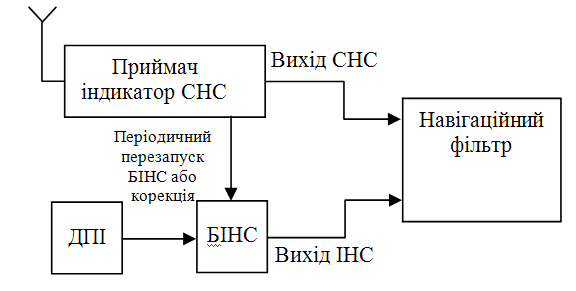
\includegraphics[scale=0.8]{sns_break}
\caption{Розімкнута схема}
\label{fig:isns_break}
\end{figure}

Періодична корекція може зводитися до періодичного перезапуску алгоритму ІНС із новими 
початковими умовами за координатами та швидкістю, дані про які надходять від приймача СНС. 
Безперервна корекція процедурно може бути оформлена як одночасна позиційна та 
швидкісна корекції ІНС за сигналами СНС. Така архітектура комплексування на  
етапі розв'язання навігаційної задачі (на етапі вторинної обробки інформації) 
забезпечує незалежність систем (крім моментів  перезапуску або корекції) й 
інформаційну надмірність сукупної структури. Вихідна інформація двох систем може 
піддаватися комплексній обробці з використанням калманівської фільтрації.

В цілому комплексна система має більш високу точність як за координатами та швидкістю, 
так і за кутовою орієнтацією. При цьому зберігається можливість одержувати позиційну, 
швидкісну та кутову інформацію (у тому числі про перевантаження та кутову швидкість), 
необхідну для цілей пілотування та навігації з високою частотою, притаманною ІНС.

Крім того, для створення  архітектури такої інтегрованої ІССН потрібні мінімальні зміни 
в апаратних засобах і програмному забезпеченні вже існуючого обладнання ЛА.

Наступною за глибиною зв'язку ІНС і СНС є слабко зв'язана система. Тут інерціальна 
система та приймач СНС як і раніше виробляють незалежні навігаційні вимірювання, 
однак з'являється з'єднувальний блок -- обчислювач ІНС СНС, у якому формується оцінка 
координат і швидкості польоту, виробляється корекція даних, отриманих від ІНС (рис. 
\ref{fig:isns_loosly}).

\begin{figure}[here]
\centering
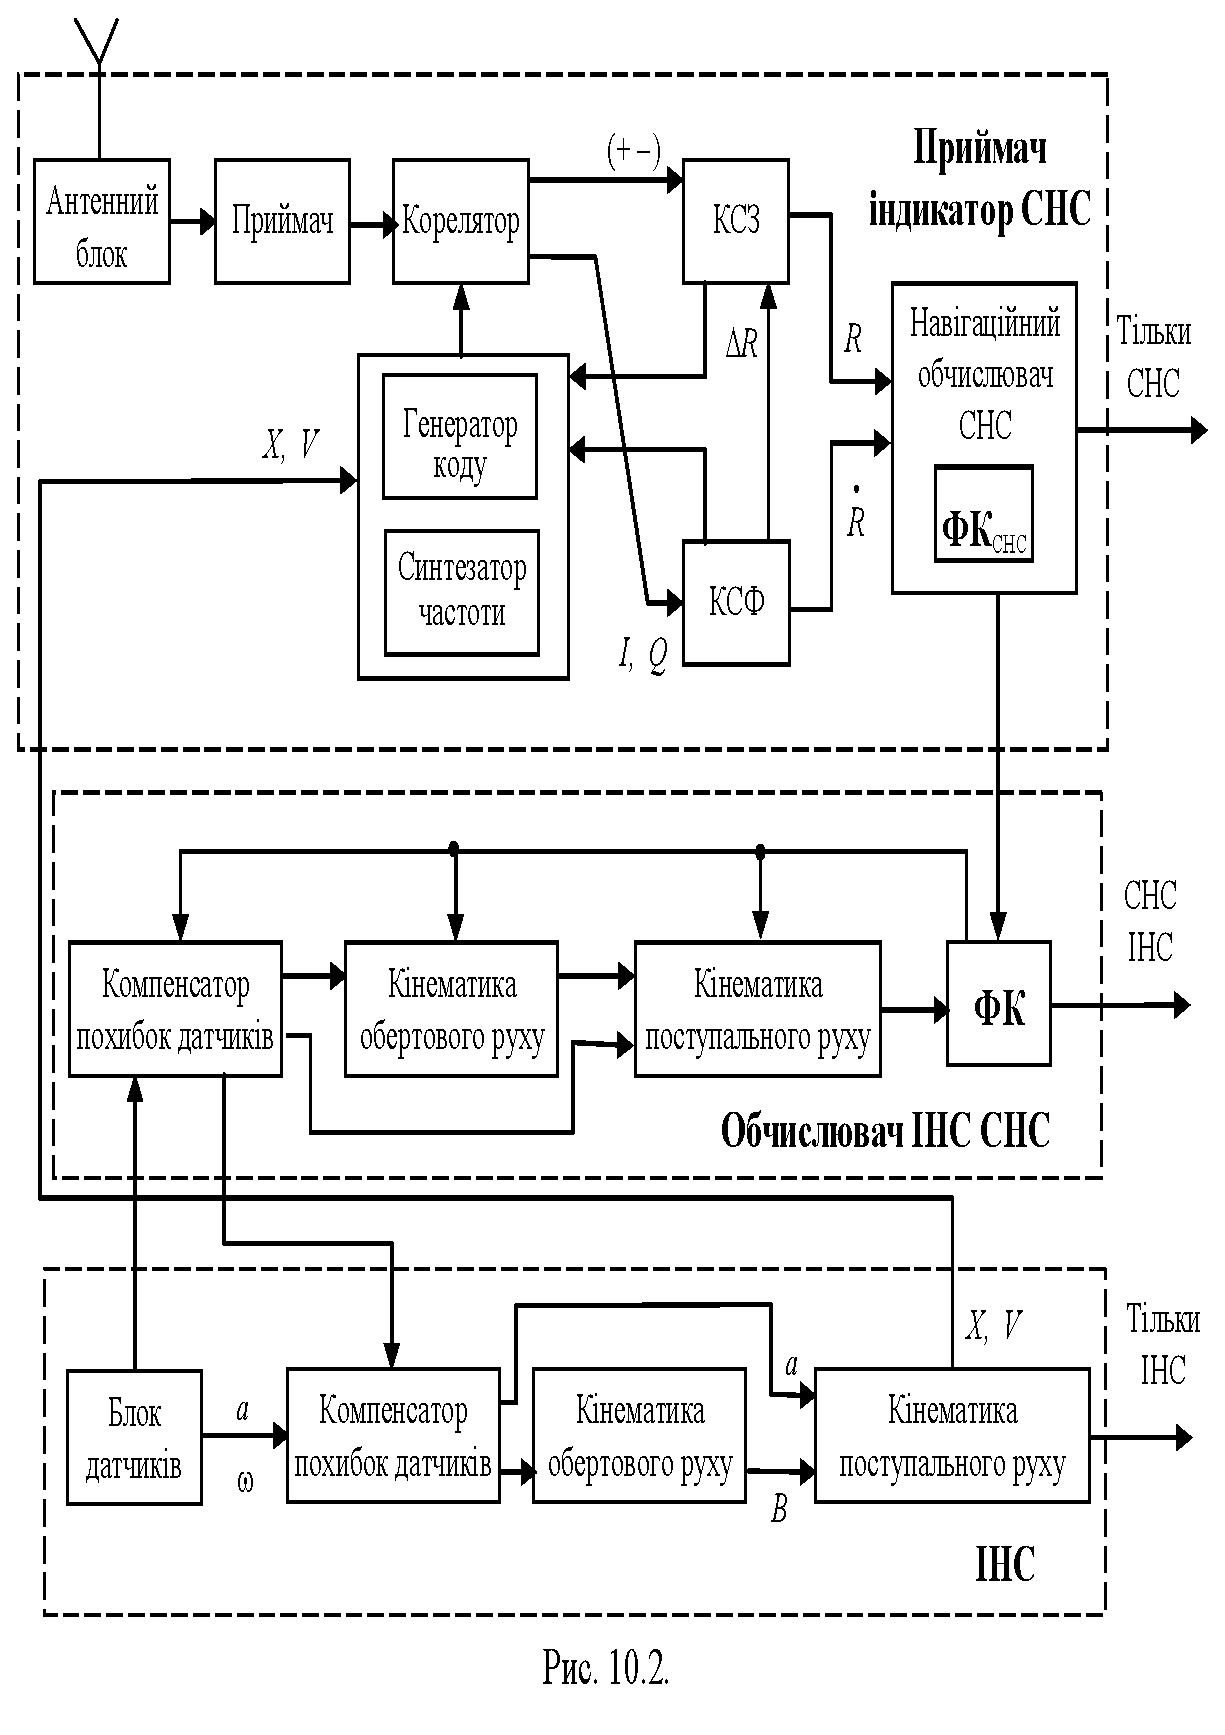
\includegraphics[bb=0mm 0mm 208mm 296mm, width=109.7mm,height=93.3mm, viewport=3mm 4mm 205mm 292mm]{isns_loosly}
\caption{Розімкнута схема}
\label{fig:isns_loosly}
\end{figure}

В цій схемі функціональний розподіл підсистем може супроводжуватися їхнім фізичним 
поділом: приймач СНС, ІНС і навігаційний обчислювач конструктивно оформляються у 
вигляді закінчених роздільних блоків, між якими організовані відповідні інформаційні 
зв'язки, що не вимагають, як правило, високих швидкостей передачі даних. Зрозуміло, 
усі три перелічені компоненти системи можуть бути розміщені й у єдиному модулі, якщо 
це бажано за умовами функціонування комплексу.

У слабко зв'язаних системах ІНС повинна забезпечити досить тривале функціонування 
зі  збереженням прийнятної точності.  Таким  чином, передбачається можливість як 
роздільного функціонування ІНС і СНС протягом тривалого періоду, так і їх сумісного 
функціонування в інтегрованому режимі. 

У СНС  (див. рис. \ref{fig:isns_loosly}) сигнал, прийнятий антенним блоком, є сигналом несучої частоти,  
модульованим за амплітудою псевдовипадковим сигналом тривалістю  $dt \approx$ 1 мксек 
(або 300 м еквівалентної довжини коду). Вхідні сигнали демодулюються і подаються 
на корелятори.  Інформація з кореляторів передається в контури слідкування за фазою 
(КСФ) і затримкою (КСЗ). Контур слідкування за затримкою видає командні сигнали, 
\nomenclature{КСФ}{контур слідкування за фазою}
\nomenclature{КСЗ}{контур слідкування за затримкою}
які здійснюють  затримку або випередження сигналів на виході корелятора (див. [+, --] 
на рис. \ref{fig:isns_loosly}) доти, поки на виході корелятора не з'явиться сигнал максимальної величини, 
а різниця сигналів корелятора на попередньому і поточному кроках не буде дорівнювати 
нулю. Це означає „захоплення'' сигналу супутника, а величина отриманої при цьому 
затримки  вважається часом поширення сигналу від супутника до приймача і використовується 
для обчислення псевдодальності $\dot{R}_{i}$ до конкретного супутника. Синфазна та 
квадратурна складові сигналів несучої частоти ($IQ$ відповідно -- на рис. \ref{fig:isns_loosly}) 
подаються в контур слідкування за фазою несучої частоти (КСФ). Арктангенс 
пропорційний амплітуді квадратурного (\textit{Q}) сигналу до синфазного (\textit{I} ) 
є похибкою КСФ. Цей сигнал похибки подається у вигляді зворотного зв'язку в корелятор, 
здійснюючи фазове автопідстроювання його частоти. Різниця частот опорного і прийнятого 
сигналів пропорційна швидкості зміни псевдодальності  $\dot{R}_{i} $. При цьому
контур КСФ має астатизм 3-го порядку, що дозволяє відслідковувати 
сигнали з постійним прискоренням (другої похідної від псевдодальності). Якщо цей 
контур захоплює і стежить за фазою, він подає коригувальний сигнал $\Delta R$ у 
контур КСЗ, підвищуючи тим самим точність визначення псевдодальності \textit{R}. 

Інформація про вимірювані псевдодальності \textit{R} і псевдошвидкості $\dot{R}_{i} $ використовується 
в алгоритмах розв'язання навігаційних задач для отримання координат і швидкості споживача, 
а також виправлень до еталона часу та частоти приймача СНС. При наявності надмірності 
з метою підвищення точності зчислення навігаційних параметрів здійснюється їхнє спільне 
оцінювання, зокрема з використанням оптимальної калманівської  фільтрації. 

Робота супутникової системи коригується від ІНС на етапі ``холодного'' і ``гарячого'' 
стартів. Тут приймач СНС використовує інформацію від ІНС тільки з метою 
більш надійного та швидкого відновлення захоплення сигналу у випадку його втрати. 
На схемі це показано зв'язком вихідного блоку ІНС і корелятора. Передана по цьому 
каналу інформація про обчислені координати та швидкість ЛА у випадку втрати слідкування 
дозволяє розрахувати оцінки передбачуваної затримки сигналу $\tau$ та доплерівського 
зсуву частоти несучої $f_{\text{доп}}$, що суттєво знижує час пошуку та захоплення сигналу. 
В результаті значно знижується час 
відновлення роботи приймача після втрати сигналу, тобто тут в деякому смислі реалізоване 
об'єднання ІНС і СНС не тільки на рівні вторинної обробки інформації, а й на рівні 
первинної обробки радіосигналів. 

У блоці ІНС на рис. \ref{fig:isns_loosly} показана структура безплатформної інерціальної системи. 
Блок датчиків видає вектори кутових  швидкостей $\omega$ та лінійних прискорень \textit{а}. 
У блоці „кінематика обертового руху'' виконується інтегрування кінематичних рівнянь 
кутового руху та формується матриця напрямних косинусів \textit{В} за інформацією 
датчиків кутових швидкостей. Матриця напрямних косинусів \textit{В} разом із даними 
акселерометрів використовується в блоці інтегрування кінематичних рівнянь поступального 
руху -- блок ``кінематика поступального руху''. На виході цього блоку формуються 
координати та швидкості ЛА у вибраній навігаційній системі.

У середній частині рис. \ref{fig:isns_loosly} зображено з'єднувальний блок -- обчислювач ІНС СНС, 
що копіює алгоритм безплатформної ІНС, здійснює в блоці „компенсатор похибок датчиків'' 
компенсацію похибок датчиків відповідно до моделей цих похибок та реалізує безпосередньо 
комплексування ІНС і СНС. Оцінка параметрів, що характеризують фазові координати 
руху ЛА, реалізується в польоті за результатами, наприклад, розширеної калманівської 
фільтрації сигналів ІНС і СНС у блоці ФК. За результатами оцінювання здійснюється 
позиційна та швидкісна корекція копії алгоритмів безплатформної ІНС. Корекція самої 
ІНС у слабко-зв'язаних системах не передбачається. Але в ІНС передбачається можливість 
компенсації інструментальних похибок вимірювальних елементів за апріорними даними 
(наприклад, за паспортними даними  системи) або за значеннями оцінок цих похибок, 
що отримані в обчислювачі ІНС СНС. В результаті в основний алгоритм ІНС передаються 
скориговані показання датчиків кутової швидкості і акселерометрів.

Як видно, у слабко зв'язаній системі навігаційні параметри, так само як і в роздільній 
схемі, виробляються незалежно як у ІНС так і в СНС, причому, як уже відзначалося, 
до складу приймача включена схема оцінювання (як правило, фільтр Калмана). Така схема 
зветься „каскадною'' через два послідовно включених фільтри Калмана. Достоїнством 
такої схеми є висока надійність інтегрованої системи, а недоліком -- взаємна кореляція 
похибок оцінок першого фільтра (фільтра супутникового приймача) і їх відмінність 
від білих шумів. Надходячи з виходу СНС на вхід другого фільтра Калмана, і стаючи 
для нього шумами вимірювань, вони порушують умови оптимальної роботи цього фільтра. 
Крім цього, у такій схемі необхідно здійснювати заходи синхронізації вимірювань ІНС 
і приймача СНС.

Підвищений рівень автономності ІНС (передбачається, що підсистема ІНС може працювати 
автономно протягом 1-ї години) вимагає значної точності інерціальних датчиків (датчиків 
кутових швидкостей і акселерометрів) і застосування досить складних алгоритмів інерціальної 
навігації. Тому такі системи досить дорогі та складні. Такі системи доцільно застосовувати 
в ПНК високої та середньої точності, але, наприклад для БПЛА, вони занадто дорогі.

У літературі можна знайти ділення слабко зв'язаних схем на три типи: стандартну, агресивну 
і так звану \textit{MAGR}-схему (\textit{Military Airborne GPS Receiver}). Відмінність 
„агресивної'' схеми від стандартної полягає в тому, що в ній використовується інформація 
БІНС про прискорення для екстраполяції навігаційних вимірювань приймача СНС в період 
між супутниковими вимірюваннями. \textit{MAGR} - схема фірми \textit{Rockwell} використовує 
інерціальні вимірювання в контурі слідкування за кодом СНС-приймача при провалі „захоплення'' 
у контурі слідкування за несучою частотою. У цьому випадку можна говорити про повноцінне 
комплексування як на рівні вторинної обробки інформації, так й на рівні первинної 
обробки інформації.

Третій варіант інтеграції систем -- жорстко зв'язана схема (рис. \ref{fig:isns_tide}).
У жорстко зв'язаних системах ступінь автономності ІНС значно менший, ніж у слабко зв'язаних 
системах: допускається автономна робота протягом від декількох секунд до декількох 
десятків секунд. Практично в цих системах ІНС найчастіше є придатком для СНС. Основна 
навігаційна інформація виробляється в СНС, у той час як ІНС інтерполює значення навігаційних 
параметрів у період між двома сусідніми тактами надходження інформації від СНС, а 
також забезпечує навігаційною інформацією системи керування польотом при короткочасній 
втраті сигналів від супутників. 

ІНС у жорстко зв'язаних системах забезпечує „сирі вимірювання''. Блок датчиків видає 
вектори кутових  і лінійних координат.  

Компенсація похибок датчиків відповідно до моделей цих похибок виконується в блоці 
компенсатора похибок від розширеного фільтра Калмана. Інтегрування кінематичних рівнянь 
обертового руху та поступального руху виконується з урахуванням скоригованих координат. 
Тобто в у жорстко зв'язаних системах виконується одночасно процедури оцінювання (фільтрації) 
і коригування ІНС.
\begin{figure}[here]
\centering
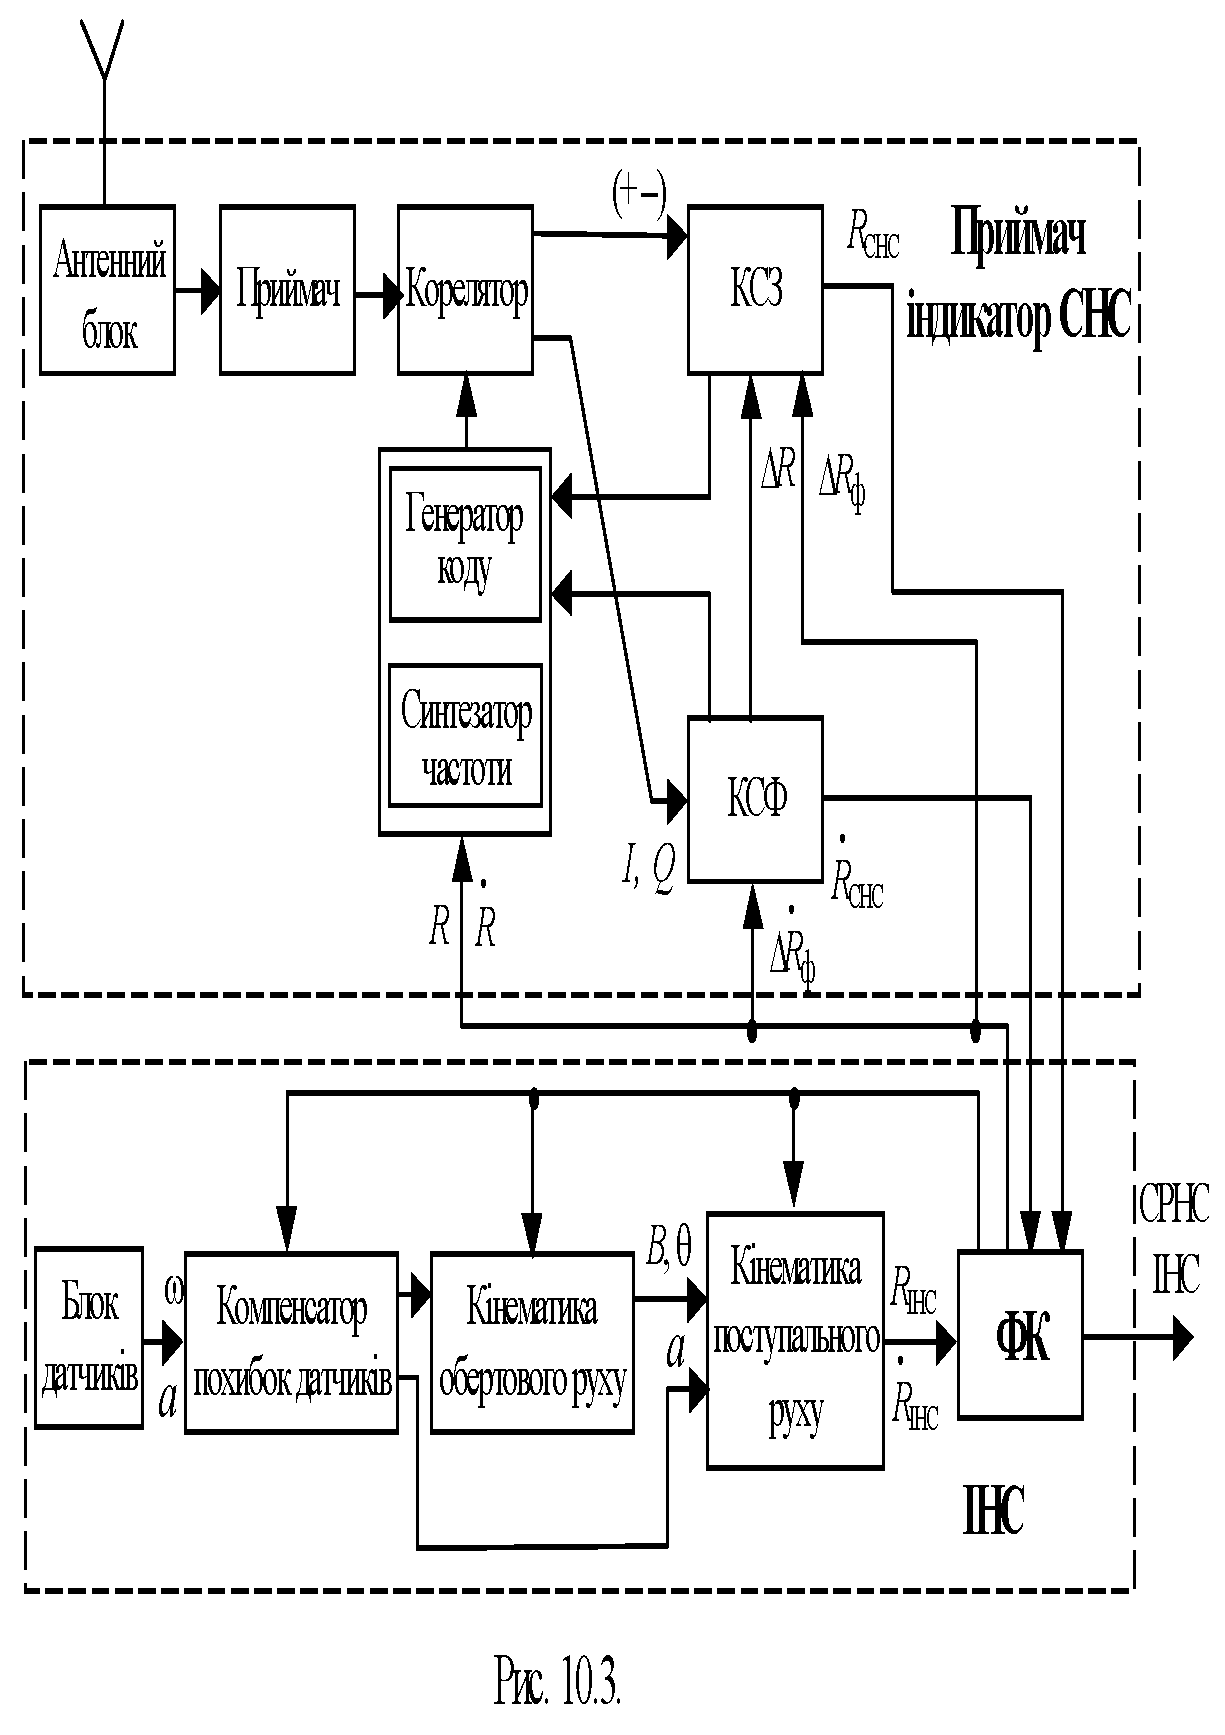
\includegraphics[bb=0mm 0mm 208mm 296mm, width=115.1mm, height=72.0mm, viewport=3mm 
4mm 205mm 292mm]{isns_tide}
\caption{Жорстко зв'язана схема інтегрування}
\label{fig:isns_tide}
\end{figure}

Приймач СНС функціонує аналогічно описаному вище варіанту 
слабко зв'язаної схеми. Відмінністю даної структури від попередніх є відсутність 
у складі приймача фільтра Калмана. У жорстко зв'язаній схемі ІНС і приймач лише забезпечують 
склад вимірювань для загального обчислювального блоку, в якому реалізований єдиний 
фільтр Калмана. Вимірювання для фільтра в жорстко зв'язаних системах будуються за 
різницею псевдодальностей або/і швидкостей зміни псевдодальностей, визначених, з 
одного боку, в ІНС за обчисленими координатами ЛА й ефемеридами супутника, і вимірюваними 
приймачем-індикатором СНС, з іншого. При цьому за навігаційну систему координат ІНС 
доцільно вибирати ту систему координат, в якій працює СНС.  

Фільтр Калмана, на відміну від попереднього випадку, повинен бути дуже швидкодіючим. 
Це пов'язано з тим, що зв'язок блока фільтра Калмана з контурами приймача СНС значно 
більш жорсткий, ніж у попередньому випадку, оскільки відмінною рисою жорстко зв'язаної 
схеми є використання контурами слідкування за затримкою і фазою інформації про розрахункові 
псевдодальності і псевдошвидкості (або про їхні збільшення), які надходить саме від 
фільтра Калмана. Використання цієї інформації дозволяє істотно поліпшити стійкість 
слідкування і знизити час відновлення роботи приймача у випадку втрати сигналів супутників. 
Необхідно, щоб ці дані надходили з високою швидкістю так, щоб період часу між вимірюваннями 
в підсистемі СНС був розбитий на велику кількість підінтервалів  з метою корекції 
контурів слідкування. Це потрібно для того, щоб постачати контуру слідкування інформацію 
навіть тоді, коли вхідний сигнал приймача відсутній або подавлений завадами, тобто 
тут реалізоване повномасштабне комплексування ІНС/СНС і на рівні первинної обробки 
інформації.

Жорстко зв'язані системи мають більшу точність при тих самих інерціальних датчиках 
у порівнянні зі слабко зв'язаними системами. У цих системах за рахунок додаткових 
сигналів корекції від  ІНС смуга пропускання контурів слідкування СНС може бути значно 
зменшена. При цьому зростає завадостійкість цих систем і зменшується ймовірність 
втрати сигналів, що відслідковуються. До того ж застосування фільтра Калмана, що 
відновлює повний вектор стану, включаючи  псевдодальність \textit{R} і швидкість 
її зміни $\dot{R}$, навіть при неповних вимірюваннях, дозволяє СНС працювати навіть 
при кількості видимих супутників менше 4-х. Якщо кількість цих супутників більше 
4-х, то фільтр Калмана здійснює комплексування інформації, що надходить від видимих 
супутників. Однак, наявність лише одного фільтра Калмана призводить до втрати надмірності 
системи, тому що стає доступним лише одне спільне рішення. 

Як і у слабко зв'язаних системах тут передбачено коригування СНС від коректованої 
ІНС на етапах „холодного'' та „гарячого'' стартів, а відновлені значення псевдодальності 
$\Delta R_{D}$ і швидкості її зміни $\Delta \dot{R}_{D} $, надходячи в контури 
слідкування за затримкою КСЗ  та за фазою КСФ сигналу СНС, забезпечують процедуру 
інтерполяції.

Таким чином, основні відмінності жорстко зв'язаної схеми від слабко зв'язаної полягають 
у наступному:

\begin{enumerate}
\item використання вихідної інформації ІНС про прискорення в контурі слідкування 
за кодом і доплерівським зсувом несучої частоти, що дозволяє звузити смугу пропускання 
контурів слідкування і підвищити швидкодію та точність настроювання;
\item використання вимірювань псевдодальностей та псевдошвидкостей (а не координат 
і швидкостей) для оцінювання похибок ІНС.
\end{enumerate}

Як вже було зазначено, жорстко зв'язані системи забезпечують більш високу точність 
розв'язання навігаційної задачі в порівнянні зі слабко зв'язаними системами. До інших 
переваг такої схеми можна віднести:

\begin{enumerate}
\item відсутність проблем взаємної кореляції шумів вимірювань та їхніх відмінностей 
від білих шумів;
\item відсутність проблеми синхронізації вимірювань ІНС і СНС, оскільки використовується 
один формувач тактових частот;
\item можливість виявлення та відбраковування схиблених вимірювань псевдодальностей 
за їхніми передбачуваними значеннями, сформованими з використанням даних від ІНС.
\end{enumerate}

До недоліків жорстко зв'язаних систем можна віднести:

\begin{enumerate}
\item необхідність розробки спеціальної апаратури споживача (приймача-індикатора СНС);
\item використання складних співвідношень для вимірювань;
\item зниження надійності, оскільки відмова ІНС призводить до відмови системи в цілому;
\item відсутність надмірності, що ускладнює рішення задач діагностики та контролю.
\end{enumerate}

Два 
останні недоліки можна усунути, використовуючи фільтр Калмана в приймачі СНС і перераховуючи 
навігаційну інформацію скоригованої ІНС у навігаційну систему координат споживача.   
Таке рішення створює деякий проміжний варіант між слабко і жорстко зв'язаними схемами -- варіант 
інерціально-супутникової системи середньої інтеграції (рис.\ref{fig:isns_lootide}) .

\begin{figure}[here]
\centering
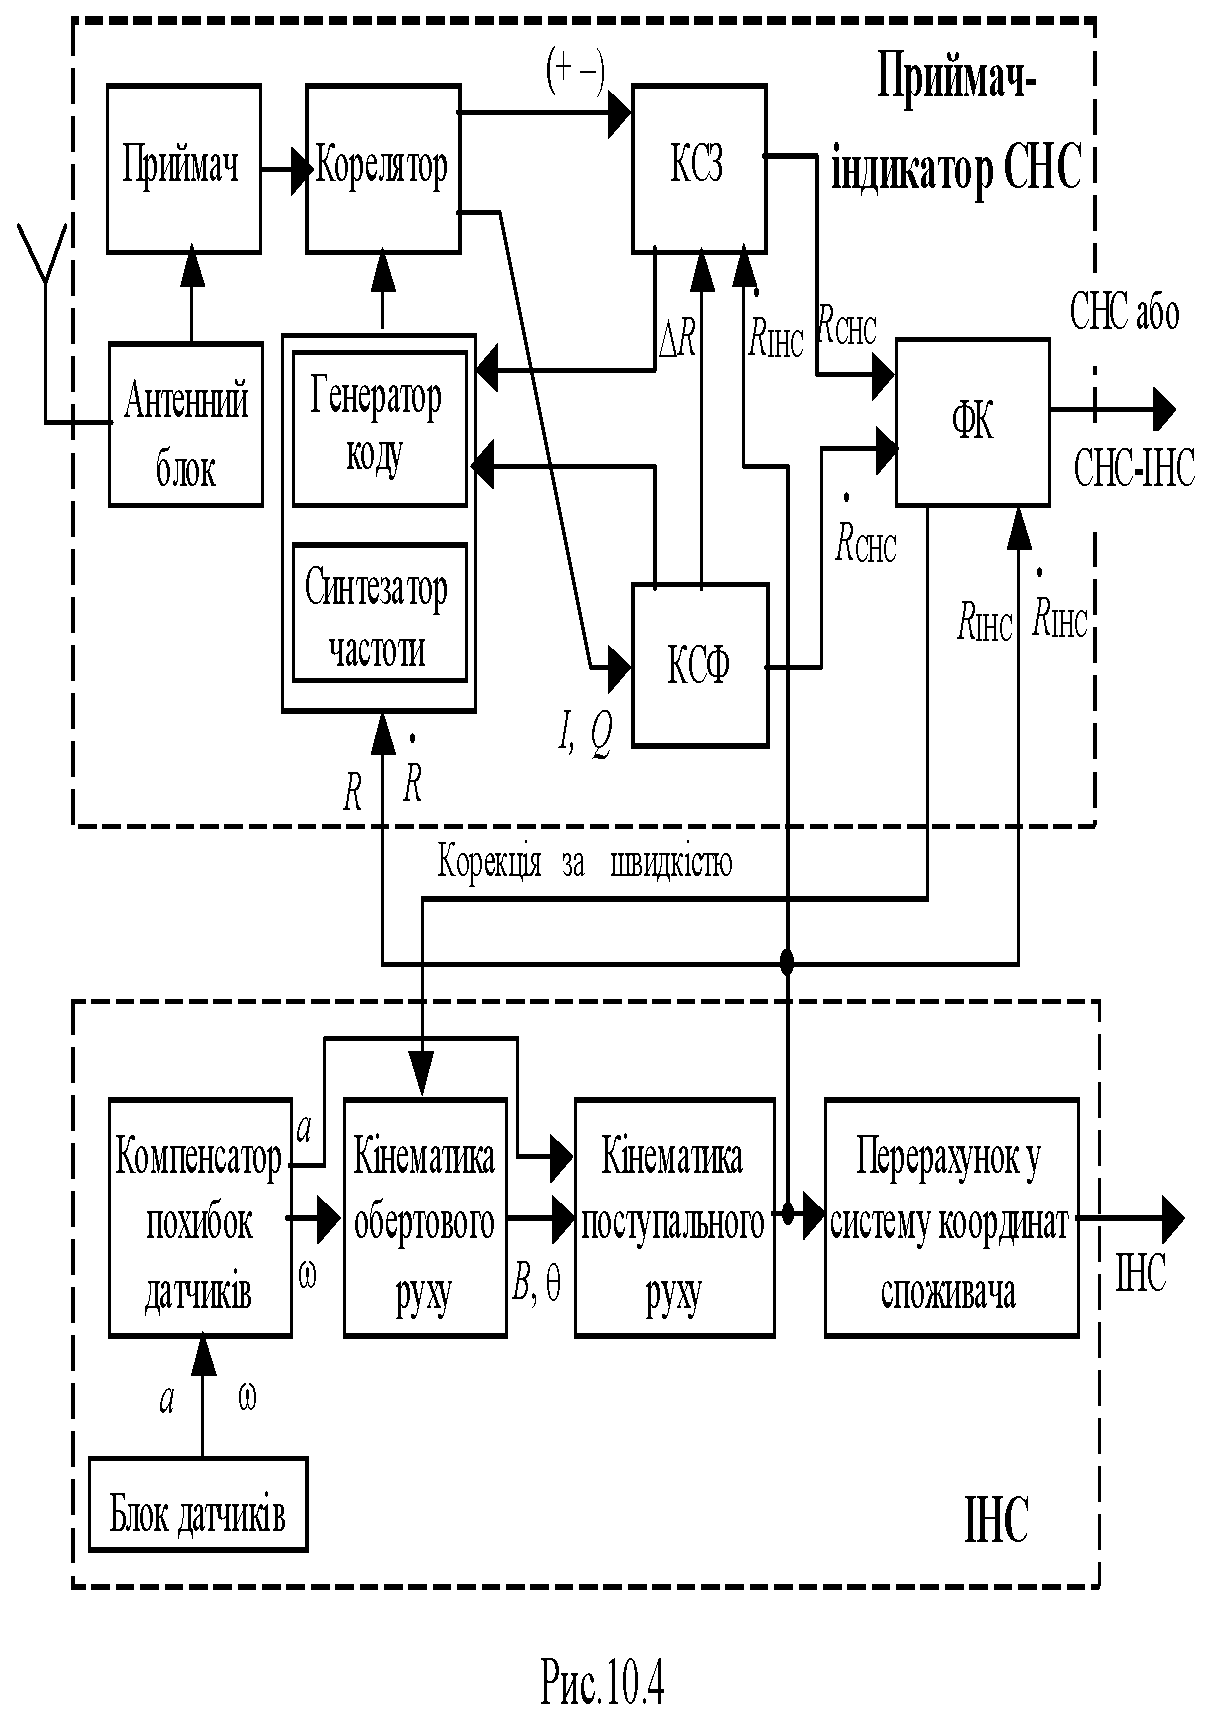
\includegraphics[bb=0mm 0mm 208mm 296mm, width=102.5mm, height=74.7mm, viewport=3mm 
4mm 205mm 292mm]{isns_lootide}
\caption{Система середнього типу інтеграції}
\label{fig:isns_lootide}
\end{figure}

Система, що зображена на рис. \ref{fig:isns_lootide}, надає два навігаційних 
рішення: одне на виході блоку СНС, інше -- на виході ІНС. Блоки, що зображені на 
схемі рис. \ref{fig:isns_lootide}, мають той же зміст, що і на попередніх схемах. ІНС може забезпечувати 
розв'язання навігаційної задачі навіть при  відсутності сигналів від СНС. Крім того, 
передбачений режим підтримки роботи СНС від ІНС за рахунок поліпшення стійкості слідкування. 
Блок КЗФ -- блок слідкування за фазою  несучої частоти, зазвичай, більш уразливий 
для природних або штучних завад. Тому, якщо цей блок слідкування втратив „захоплення'' 
фази і не виконує функцію підтримки слідкування КЗС, тобто працює тільки блок КСЗ - 
блок слідкування за затримкою, то ІНС заміняє відсутній сигнал $\Delta$\textit{R} на 
сигнал $\dot{R} $, підтримуючи, таким чином, роботу супутникової системи 
без збоїв.

ІНС у цьому випадку, так само як і у всіх інших, використовується також і для екстраполяції 
сигналів положення \textit{R} і швидкості $\dot{R}$між двома вимірюваннями СНС.

Оскільки у фільтрі Калмана відновлюється цілком весь вектор стану ЛА, то  змінні 
кутової орієнтації використовуються для корекції алгоритмів інтегрування кінематичних 
рівнянь кутового руху, тобто здійснюється корекція за швидкістю. 

Крім розглянутих варіантів структур комплексної системи, існують ще й інші варіанти, 
що побудовані як за принципом слабкої, так і жорсткої інтеграції. Але при цьому слід 
мати на увазі, що ці варіанти вимагають значно більш складного і дорогого математичного 
забезпечення в порівнянні з уже розглянутими варіантами структур.  

Так звані глибоко інтегровані системи є ще більш складними і менш гнучкими з огляду 
організації їхньої структури, мають жорстку організацію зв'язків і єдиний вихід (рис. 
\ref{fig:isns_heavytide}). 

\begin{figure}[here]
\centering
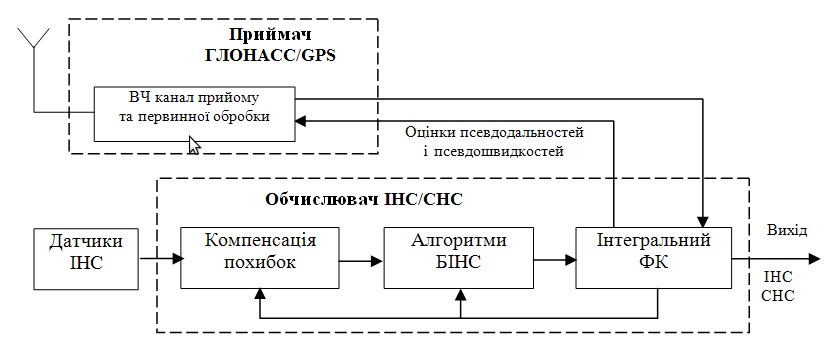
\includegraphics[scale=0.45]{isns_heavytide}
\caption{Глибоко інтегрована схема}
\label{fig:isns_heavytide}
\end{figure}

Обчислювач ІНС/СНС реалізує алгоритми безплатформної ІНС й алгоритми оптимальної 
оцінки параметрів. Всі оцінки виробляються в інтегральному фільтрі Калмана, а приймач 
СНС ГЛОНАСС/GРS ще більш спрощується. У цій схемі він складається тільки з високочастотного 
каналу прийому і первинної обробки інформації, що включає високочастотний прийомний 
тракт, генератор коду, корелятори і схему „захоплення''. Виходи кореляторів є входами 
для інтегрального фільтра Калмана, де обчислюються не тільки похибки ІНС, але й оцінки 
псевдодальностей і псевдошвидкостей, які передаються в приймач для поліпшення характеристик 
„захоплення'' сигналу. Таким чином, традиційні контури слідкування за кодом і доплерівською 
частотою включаються в загальний інтегральний фільтр комплексної системи. У такій 
схемі фільтр повинен мати двадцятий-сороковий порядок, і для його реалізації потрібна 
БЦОМ із високою швидкодією.

Усі перераховані схеми комплексування СНС і ІНС (крім першої), одержують на виході 
фільтра Калмана оцінки інструментальних похибок ІНС (похибки зсуву нулів гіроскопів 
і акселерометрів, похибки масштабних коефіцієнтів і т. ін.), які використовуються 
для корекції інерціальних датчиків. Тому при перервах надходження даних із приймача 
отримані раніше оцінки похибок ІНС і її вимірювальних елементів дозволяють поліпшити 
точнісні характеристики ІНС в автономному режимі.

В табл. \ref{tab:compare} підсумовані основні особливості перелічених схем комплексних систем.

\begin{table}[here]
\centering
\caption{Особливості схем комплексування}
\label{tab:compare}
\begin{tabular}{|p{30mm}|p{110mm}|} \hline 
Тип системи & Основні особливості \\ \hline 
Роздільна & Надмірність, обмеженість похибок оцінок місця розташування і швидкості, 
наявність інформації про орієнтацію і кутову швидкість, висока швидкість видачі інформації, 
мінімальні зміни в бортовій апаратурі  \\ \hline 

Слабко\newline зв'язана & Усі перераховані особливості роздільних систем, плюс більш 
швидке відновлення слідкування за кодом і фазою сигналів СНС, виставлення та калібрування 
БІНС у польоті, як наслідок -- підвищена точність під час відсутності сигналу СНС  \\ \hline 

Жорстко зв'язана & Подальше поліпшення точності і калібрування, підвищена стійкість слідкування 
за сигналами СНС при маневрах ЛА, підвищена завадостійкість  \\ \hline
 
Глибоко інтегрована & Достоїнства: єдиний фільтр усуває проблему ``каскадного'' включення 
фільтрів, компактність, знижені вимоги з енергозабезпечення. Недоліки: вектор стану 
містить до 40 компонентів, тому фільтр складно реалізувати; необхідність розробки 
спеціальних датчиків  \\ \hline 
\end{tabular}
\end{table}

Перші дві з приведених структур інтегрованих систем можуть бути реалізовані з використанням 
існуючих супутникових приймачів та інерціальних систем. Разом з тим жорстко зв'язана 
і особливо глибоко інтегрована схеми в обов'язковому порядку потребують розробки 
спеціальних приймачів і обчислювачів супутникової навігації для забезпечення корекції 
обох контурів спостереження від інерціальної системи навігації, а також створення 
спеціалізованих датчиків для інерціальних систем, виготовлених на одній технологічній 
та конструктивній базі. При цьому можуть бути використані самі передові технології, 
наприклад мікромеханічні датчики. Це дозволяє одержати інтегровані системи менших 
габаритів, маси, енергоспоживання. Але з точки зору розробника ці обставини є певним 
недоліком таких систем. 

Об'єктом, на який передбачається встановлювати інтегровану навігаційну систему є пасажирський середньомагістральний літак українського виробництва, через це обираємо  слабкозв’язану схему комплексування, оскільки архітектура такої інтегрованої КІССН потрібує мінімальної зміни в апаратних засобах і програмному забезпеченні складових систем комплексної системи. Це дає можливість використовувати надійні, покупні і уніфіковані блоки системи і легко розширяти навігаційне забезпечення додаючи нове обладнання. До того ж вихідна інформація двох систем може просто піддаватися комплексної обробці з використанням тих чи інших алгоритмів оптимальної фільтрації. Окрім цього структурна надмірність надає більшу надійність системи: вихід однієї підсистеми з ладу не впливає на роботу іншої (на відміну з жорстко зв’язаною схемою).

Отже після вибору методу комплексування, необхідно визначитись з варіантами супутникової та інерціальної навігаційної системи, які б оптимально підходили під вибрану архітектуру побудови.


\subsection{Аналіз та вибір варіанта супутникової навігаційної системи}

На сьогодні має сенс розглядати лише дві супутникові навігаційні системи : GPS (Global Positioning System), 
ГЛОНАСС (Глобальна Навігаційна Супутникова Система).

Двадцять чотири супутники системи GPS знаходяться на 12-годинних орбітах висотою 
20146 км із нахиленням орбіти, рівним 55. Таким чином, 
у будь-якій крапці земної кулі в межах прямої видимості мається не менш чотирьох супутників 
у конфігурації, сприятливої для місцевизначення.

Система заснована на обчисленні відстані від користувача до супутника за обмірюваним часом 
від передачі сигналу супутником до прийому цього сигналу користувачем.

Глобальна Навігаційна Супутникова Система (ГЛОНАСС) -- це технології російських конструкторів і вчених.
Вона складається 
з 21 супутників, що, знаходячись у заданих крапках на високих орбітах, безупинно випромінюють 
убік Землі спеціальні навігаційні сигнали. Будь яка людина або транспортний засіб, оснащені 
спеціальним приладом для прийому й обробки цих сигналів, можуть з високою точністю в 
будь-якій крапці Землі і навколоземного простору визначити власні координати і швидкість 
руху, а також здійснити прив'язку до точного часу.

У складі сучасної супутникової радіонавігаційної системи (СРНС) типу ГЛОНАСС і
\nomenclature{СРНС}{супутникова радіонавігаційна система} 
GPS функціонують три основні підсистеми:

\begin{enumerate}
\item Підсистема космічних апаратів (ПКА), що складається з навігаційних супутників (НС)
\nomenclature{ПКА}{підсистема космічних апаратів} 
\nomenclature{НС}{навігаційний супутник} 
(мережа навігаційних супутників - космічний сегмент). ПКА СРНС складається з визначеного 
числа навігаційних супутників. Основні функції НС --- формування і випромінювання 
радіосигналів, необхідних для навігаційних визначень споживачів СРНС, контролю бортових 
систем супутника підсистемою контролю і керування СРНС. Відповідні характеристики сигналів 
НС і способи їхньої обробки дозволяють проводити навігаційні виміри з високою точністю.
 \item Підсистема контролю і керування (ПКК) (наземний командно-вимірювальний комплекс (КВК)) - 
\nomenclature{КВК}{командно-вимірювальний комплекс}
\nomenclature{ПКК}{підсистема контролю і керування}
сегмент керування. ПКК являє собою комплекс наземних засобів, що забезпечують 
спостереження і контроль за траєкторіями руху НС, якістю функціонування їхньої апаратури, 
керування режимами її роботи і параметрами супутникових радіосигналів, складом, обсягом і 
дискретністю переданої із супутників навігаційної інформації та ін.
\item Апаратура споживачів (АС) СРНС (прийомоіндикатори (ПІ)) - сегмент споживачів.
\nomenclature{ПІ}{прийомоіндикатор}
Апаратура споживачів призначена для визначення просторових координат, вектора швидкості, 
часу й інших навігаційних параметрів у результаті прийому й обробки радіосигналів багатьох 
навігаційних супутників.
\end{enumerate}

На вхід ПІ надходять сигнали від НС, що знаходяться в зоні радіо видимості. Оскільки для 
рішення навігаційної задачі необхідно вимірити псевдодальності і псевдошвидкості відносно, 
як мінімум, чотирьох НС, то ПІ повинний бути багатоканальним (більш 24 у сполучених ГЛОНАСС і GPS ).

Сучасні ПІ є аналого-цифровими системами, що здійснюють аналогову і цифрову обробку 
сигналів. Перехід на цифрову обробку здійснюється на одній із проміжних частот, при 
цьому має місце тенденція до підвищення цієї проміжної частоти.
\nomenclature{АБ}{антенний блок}

Основа типового варіанту ПІ -- два конструктивно роздільних блоків: антенний блок (АБ) та 
прийомообчислювач (ПО), які призначені для прийому й обробки навігаційних сигналів 
супутників з метою визначення необхідної споживачам інформації (просторово-тимчасових 
координат, напрямки і швидкості і т.п.).

В антенному блоці (рис. \ref{fig:ant_sns}) сукупність сигналів НС, прийнятих антеною, попередньо 
підсилюється і фільтрується по всій смузі несучих частот НС у попередньому підсилювачі 
(ПП) зі смуговим фільтром (СФ). \nomenclature{СФ}{смуговий фільтр}
\begin{figure}[here]
\centering
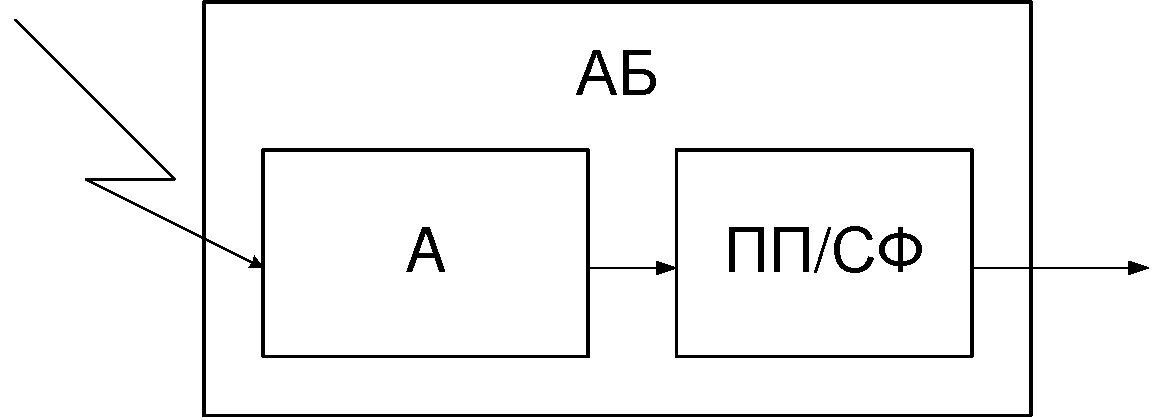
\includegraphics[scale=0.4]{ant_sns}
\caption{Схема антенного блоку СНС}
\label{fig:ant_sns}
\end{figure} 

Прийомообчислювач виконаний у вигляді блоку, у якому розташовані модулі вторинних 
джерел живлення і плати --- прийомокорелятора, навігаційного обчислювача та інтерфейсного 
пристрою (рис. \ref{fig:sns}). Вхід ПО через фідерну лінію з'єднаний з виходом антенного блоку. 
В аналоговому приймачі АП сигнали підсилюються, фільтруються і переносяться з несучої 
частоти на проміжну (зниження частоти). В аналого-цифровому перетворювачі АЦП аналоговий
\nomenclature{СФ}{смуговий фільтр}
сигнал перетвориться в цифрову форму.
\begin{figure}[here]
\centering
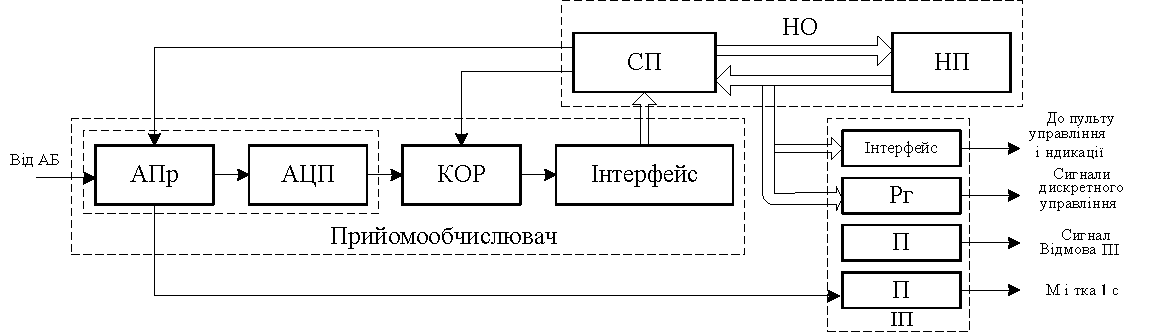
\includegraphics[scale=0.9]{sns}
\caption{Схема прийомообчислювача}
\label{fig:sns}
\end{figure} 
В кореляторі (КОР) у цифровій формі формуються синфазні  і квадратурні  відліки, що є 
основою роботи алгоритмів пошуку сигналів по затримці і частоті спостереження за псевдодальністю, 
фазою сигналу і виділення навігаційного повідомлення.

Навігаційний обчислювач НО є цифровим процесором, у якому реалізується обчислювальний процес 
і керування роботою ПІ. Навігаційний обчислювач зручно представити у виді сигнального процесора 
СП, що реалізує алгоритми первинної обробки квадратурних складових, і навігаційного процесора 
НП, що реалізує алгоритми низькочастотної обробки, тобто рішення навігаційної задачі.

У прийнятого радіосигналу виміряються затримка $\tau$ або доплерівський зсув частоти $f_{\text{доп}}$, 
які є радіонавігаційними параметрами, а відповідні їм дальність до об'єкта $D=c*\tau$  
і радіальна швидкість зближення $V_{p}=f_{\text{доп}}\lambda$   служать навігаційними параметрами 
(\textit{с } -- швидкість світла;$\lambda$ -- довжина хвилі радіосигналу).

Просторове положення споживача визначається в прийомоіндикаторі в два етапи: спочатку визначаються 
поточні координати супутників і первинні навігаційні параметри (дальність, її похідні й ін.) щодо 
відповідних НС, а потім розраховуються вторинні --- географічна широта, довгота, висота споживача і т.д.

Вектор швидкості споживача обчислюють шляхом обробки результатів вимірів доплерівських зсувів 
частоти сигналів НС з урахуванням відомого вектора швидкості супутника. 

Інтерфейсний пристрій (ІП) призначений для забезпечення взаємодії прийомоіндикатора з зовнішніми 
пристроями такими, наприклад, як пульт керування й індикації (ПКІ). Додатково до складу ІП входять 
два підсилювачі П, що формують ознаку відмови ПІ і сигнали дискретного керування, а також 8-розрядний 
регістр Рг, що приймає сигнали дискретного керування. Цей регістр доступний для читання з боку НО. 
Останній, у залежності від інформації, що знаходиться в регістрі, вибирає той або інший режим роботи.

Таким чином, основною операцією, що виконуваної в СНС за допомогою космічного сегменту, сегменту 
керування та сегменту споживача, є визначення просторових координат місця розташування споживачів і 
часу, тобто просторово-тимчасових координат (ПТК). Як було показано, цю операцію здійснюють відповідно 
до концепції незалежної навігації, що передбачає обчислення шуканих навігаційних параметрів 
безпосередньо в апаратурі споживача. У рамках цієї концепції в СРНС обраний позиційний спосіб 
визначення місця розташування споживачів на основі беззапитних (пасивних) далекомірних вимірів по 
сигналах декількох навігаційних штучних супутників Землі з відомими координатами. Висока точність 
визначення місця розташування споживачів обумовлена багатьма факторами, включаючи взаємне розташування 
супутників і параметри їхніх навігаційних сигналів. Структура космічного сегмента забезпечує для 
споживача постійну видимість необхідного числа супутників.

Використання СНС в інтересах місцезнаходження і навігації рухливих об'єктів, а також у рішенні 
спеціальних задач (спостереження, аерофотознімання, пошук корисних копалин, пошук і порятунок 
транспортних засобів, що терплять нещастя, і людей) висуває високі вимоги.

Вимоги до точнісних характеристик, таких як середньоквадратичне відхилення помилки (СКП) визначення 
навігаційних параметрів, показників надійності навігаційного забезпечення, тощо наступні:
\begin{itemize}
  \itemдоступність (готовність),  мірою якої є імовірність працездатності СРНС перед виконанням 
тієї або іншої задачі та у процесі її виконання. Чисельні значення доступності складають 0,95...\dots 0,997;
 \itemцілісність, мірою якої є імовірність виявлення відмови протягом часу, рівному заданому 
або менше. Вимоги до цілісності для маршрутних польотів складає 0,999;
 \itemбезперервність обслуговування, мірою якої служить імовірність працездатності системи 
протягом найбільш відповідальних відрізків часу. На етапах заходу на посадку вимоги до безперервності 
обслуговування складають $10^{-5}$ \dots ... $10^{-4}$ для проміжків часу від 15 до 150 с.
\end{itemize}

Основні навігаційні параметри, що визначаються в СРНС -- дальність і радіальна швидкість. Відповідними 
їм радіонавігаційними параметрами (параметрами радіосигналу) служать затримка t сигналу і доплерівський 
зсув частоти $f_\text{доп}$. Оскільки головною вимогою до СРНС є висока точність виміру 
навігаційних параметрів, отже, й основною вимогою до радіосигналів так само є висока точність 
виміру затримки t сигналу і доплерівського зсуву частоти $f_\text{доп}$.

Вимоги до підвищення точності затримки сигналу і доплерівського зсуву частоти суперечливі. 
Для підвищення точності виміру затримки необхідно розширювати спектр сигналу, а для підвищення 
точності виміру  доплерівського зсуву частоти --  збільшувати тривалість сигналу.

Дане протиріччя вирішується при вирішенні задачі спільної оцінки t та  $f_\text{доп}$.

Підвищення точності спільних оцінок затримки сигналу і доплерівського зсуву частоти можна 
досягти за рахунок збільшення так званої  бази сигналу -- \textit{В}(добуток ефективної 
тривалості сигналу на ефективну ширину спектра сигналу) і основною вимогою до радіосигналів у 
СРНС є збільшення бази сигналу $В>>1$. Такі сигнали називають шумоподібними. 
Відомо, що стійкість до перешкод радіотехнічної системи визначається значенням бази сигналу, 
а для більшості ЛА скритність і перешкодозахищеність є одним з визначальних вимог. 

Інша істотна вимога --- забезпечення багатостанційного доступу. При визначенні навігаційних 
параметрів у споживача повинна бути можливість одночасного доступу до сигналів від різних 
супутників. Проблема багатостанційного доступу вирішується шляхом тимчасового, частотного 
або кодового поділу сигналів, наприклад, у супутниковій навігаційній системі GPS використовується 
кодовий поділ, у СРНС ГЛОНАСС - частотний.

З результатів аналізів стає очевидно, що не має принципової різниці між супутниковими 
навігаційними системами GPS та ГЛОНАСС.

В залежності від області використання апаратура споживача (АС) має свої особливості, 
тому виробники АС завжди вказують на область застосування відповідного зразка. Крім 
основних блоків, таких, як антена, приймач, індикатор, АС може містити допоміжні, що 
забезпечують виконання спеціальних сервісних функцій, наприклад, діагностику вузлів 
транспортного засобу, зв'язок з диспетчерським пунктом і т.п.

З огляду на, те що  супутникова система навігації буде працювати в комплексі з 
інерціальною системою навігації, то навряд варто встановлювати  на борт ЛА повний 
комплект супутникової системи. Досить обмежитися  прийомоіндикатором і сигнальним 
процесором, думаючи, що алгоритми рішення навігаційної задачі будуть вирішуватися 
в спільному процесорі інерціально - супутникової системи навігації. 

Виходячи з вищенаведеного, а також враховуючи умови застосування ЛА та вимоги 
ТЗ можна сформулювати вимоги, яким повинний задовольняти обраний тип прийомоіндикатора 
СРНС. 

Розв'язувані задачі:
\begin{itemize}
\item автоматичне, безперервне, глобальне, всепогодне визначення поточних ЗD-координат 
місця розташування, вектора шляхової швидкості шляхового кута ЛА при роботі: по 
сигналу стандартної точності частотного діапазону L1 ГЛОНАСС; по сигналі З/А-коду 
GPS; при спільній обробці вищевказаних сигналів;
\item видача поточних ЗD-координат місця розташування ЛА, що є складовими вектора 
швидкості і шляхового кута в системі координат СК-42 або ПЗ-90 у географічному 
форматі, а також ознак режиму роботи апаратури;
\item стійке визначення навігаційних параметрів при русі з лінійними прискореннями 
і при стрибкоподібних змінах прискорення;
\item  можливість переключення з антени носія на антену ЛА; 
\item інтегральна оцінка очікуваної точності визначення поточних координат місця розташування;
\item автоматичний вибір оптимального з погляду очікуваної точності сузір'я НС ГЛОНАСС і GPS при роботі в сполученому режимі;
\item автоматичне рішення навігаційної задачі в географічній системі координат:  
\end{itemize}

З огляду на зазначені вимоги можна запропонувати СНС типу --- SPIRIT 24 Channel
GPS+GLONASS Receiver DuoStar-1000 (рис.\ref{fig:glo_gps_duostar1000}). Приймач працює одночасно з системами GPS та ГЛОНАСС, добре себе зарекомендував в роботі на рухомих динамічних об’єктах (із значними прискореннями та різкими поштовхами), високим рівнем вібрацій та в широкому діапазонів температурних умов.
\begin{figure}[here]
\centering
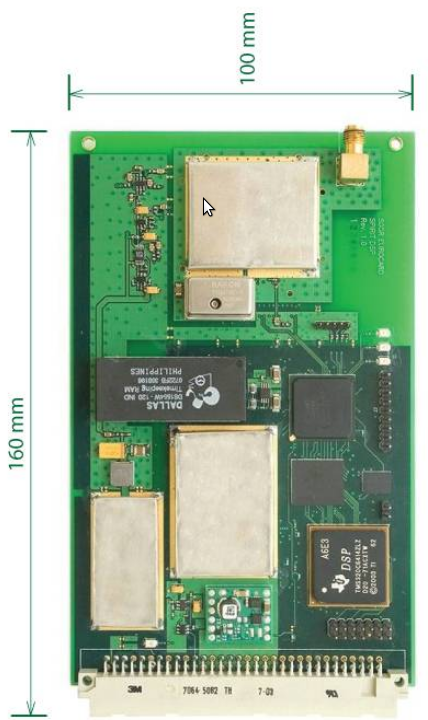
\includegraphics[scale=0.45]{glo_gps_duostar1000}
\caption{СНС приймач SPIRIT DuoStar-1000}
\label{fig:glo_gps_duostar1000}
\end{figure} 

Комбінування GPS та ГЛОНАСС дає можливість використовувати практично до 56 супутників (32 GPS та 24 ГЛОНАСС). В цьому випадку приймач подівійної системи може використовувати всі видимі супутники (до 24), що позитивно позначається на надійність та стабільність роботи в місцях з обмеженою видимістю.

\begin{table}[here]
\small
\caption{SPIRIT 24 Channel GPS+GLONASS Receiver DuoStar-1000}
\centering
\begin{tabular}{|p{60mm}|p{60mm}|} \hline 
 Параметр & Значення\\ \hline 
 Частоты & GPS L1 та ГЛОНАСС L1\\ \hline 
 Кількість каналі & 24\\ \hline 
 Протоколи передачі & NMEA 0183 v.2.3, RTCM SC104 v.2.2\\ \hline 
 Позиційна точність & 5 м \\ \hline 
 Точність визнач. часу & 30 нс. \\ \hline 
 Точність визнач. швидкості & 0.05 м/с \\ \hline 
 Динаміка & 20g \\ \hline 
 Гарячий старт & 1 с \\ \hline 
 Холодний старт & 30 с \\ \hline 
 Частота вихідного сигналу & 10 Гц \\ \hline 
\end{tabular}
\label{tb:ac}
\end{table}

Наступним кроком є вибір інерціальної навігаційної системи, яка разом з СНС є ядром комплексної навігаційної системи. Тільки поєднання цих двох підсистеми, дає можливість задовольнити вимоги точності та надійності.

\subsection{Вибір варіанту побудови інерціальної навігаційної системи}

В інерціальній  навігаційній системи (ІНС)  інформацію про швидкість і 
координати одержують шляхом інтегрування сигналів, що відповідають прискоренням 
ЛА. Інформація про прискорення надходить від розташованих на борту ЛА 
акселерометрів. Процедура інтегрування векторних величин, якими є прискорення і 
швидкості ЛА, забезпечується шляхом відтворення (моделювання) на борті ЛА відповідної 
системи координат. З цією метою найчастіше використовують гіростабілізатори 
або гіроскопічні датчики кутової швидкості разом з обчислювачем. 

Наявність похибок датчиків ІНС у свою чергу приводить до похибок 
у визначенні навігаційних координат руху ЛА, от чому при створенні 
ІНС намагаються зменшити величину похибок первинних датчиків.
Перевагами інерціальних систем перед іншими системами навігації є їхня 
повна автономність, абсолютна перешкодозахищеність, а також висока інформативність.
У залежності від способів розташування акселерометрів на ЛА розрізняють платформні 
і безплатформні ІНС. У першому випадку акселерометри встановлюються на 
гіростабілізуючій платформі, у другому безпосередньо на корпусі ЛА або в 
спеціальному блоці чуттєвих елементів, при цьому осі чутливості акселерометрів 
не змінюють орієнтацію відносно напрямку осей, зв'язаних з ЛА.
Серед платформних ІНС розрізняють ІНС з некоректованою платформою та 
ІНС з горизонтальною платформою. 

У ІНС з некоректованою платформою осі платформи, а також акселерометри, що установлені на 
цій платформі, не обертаються в інерціальному просторі. 
ІНС з горизонтальною платформою у свою чергу класифікують як ІНС із вільною в 
азимуті платформою (платформа розташовується відносно точки світового простору – відносно зірки) 
та ІНС з корегованою в азимуті платформою (платформа стабілізується відносно меридіана – „направлена” на північ).
По ролі обчислювача у визначенні кутових і лінійних координат прийнято 
розрізняти геометричні, напіваналітичні та аналітичні ІНС. У геометричних ІНС 
основним елементом служить гіростабілізатор, що відтворює напрямок осей інерціальної 
системи відліку, і платформа з акселерометрами, осі чутливості яких відтворюють деякі 
напрямки в площині обрію і напрямок місцевої вертикалі. Роль обчислювача в такій ІНС 
мінімальна і зводиться до забезпечення корекції заданого положення платформи. Інформація 
про координати знімається з кутомірних пристроїв гіростабілізатора і платформи.

До напіваналітичних систем відносять системи з горизонтальною платформою. У 
цих системах гіроплатформа з акселерометрами відтворює напрямок нормальної (рухливої) 
системи відліку. З кутомірних пристроїв гіростабілізатора знімається інформація про 
кути крену, тангажу, курсу ЛА. Обчислювач ІНС вирішує задачу визначення кінематичних 
параметрів руху центра мас ЛА і видає сигнали для корекції гіростабілізатора.
До аналітичних ІНС відносять безплатформні ІНС та ІНС з акселерометрами на некоректованому 
або вільному гіростабілізаторі. Обчислювач ІНС у даному випадку виконує найбільший обсяг 
обчислень. Крім визначення кінематичних параметрів руху центра мас ЛА він визначає кутову 
орієнтацію нормальної рухливої системи координат відносно інерціальної і кутову орієнтацію 
зв'язаної рухливої системи координат щодо нормальної. 

Побудова прецизійних і одночасно надійних гіроплатформ являє собою складну технічну задачу. 
Тому останнім часом усе більше уваги приділяється розробці так званих безплатформних ІНС (БІНС), 
у яких датчики акселерометрів жорстко зв’язані з корпусом ЛА. Такі системи мають у своєму складі 
гіроскопічні прилади, але головною задачею цих пристроїв є забезпечення обчислювачів БІНС 
інформацією про кутове положення ЛА, а так само про положення осей чутливості акселерометрів 
відносно обраної навігаційної системи координат. Відсутність горизонтальної платформи вимагає 
виділяти з показань акселерометрів сигнали, що є прискореннями ЛА, тобто обчислювачі БІНС 
аналітично визначають напрямок вертикалі. При цьому точність зазначеного моделювання 
визначається точністю роботи обчислювача і, природно, точністю датчиків первинної навігаційної інформації.
До числа потенційних переваг безплатформних інерціальних навігаційних систем БІНС у 
порівнянні з платформними ІНС можна віднести:

\begin{itemize}
 \item менші розміри, вага й енергоємність;
 \item істотне спрощення механічної частини системи ; 
 \item відсутність обмежень по кутах розвороту;
 \item скорочення часу початкової виставки.
\end{itemize}

Тому, навіть за певних труднощів, що виникають при створенні БІНС, таких як:
\begin{itemize}
%  \item 
 \item розробка датчиків інформації із широким діапазоном вимірів і прийнятною точністю в умовах їхнього твердого кріплення на борті ЛА;
 \item розробка БЦВМ, що мають достатню швидкодію.
\end{itemize}

У роботі розглядатиметься безплатформна інерціальна система.
В залежності від способу визначення кутового положення об'єкта в інерціальному просторі 
можливі наступні основні варіанти схеми БІНС:

Перший варіант передбачає наявність у БІНС шести акселерометрів  рознесених по осям об'єкта на відстань 
(для виміру кутових прискорень) і обчислювального пристрою (ОП);

Другий варіант включає три лінійних акселерометри  і три вимірники кутової 
швидкості руху об'єкта щодо центра мас, встановлених в центрі мас об'єкта, а також ОП.

Третій варіант передбачає наявність трьох лінійних акселерометрів, і вимірника 
кутового положення об'єкта в інерціальному просторі, встановлених у центрі мас об'єкта, і ОП.

Стосовно розглянутого класу ЛА використання БІНС першого варіанту зустрічає складності 
реалізації через малу вимірювальну базу  визначення кутових прискорень об'єкта за 
допомогою акселерометрів. До того ж, похибки БІНС цього варіанту у визначенні координати, 
обумовлені помилками виміру кутових прискорень, має три складових: одна з них постійна, 
інша наростає пропорційно квадратові часу руху, а третя змінюється з періодом Шулера. 
Звідси ясно, що цей варіант схеми може бути застосований тільки при досить точних 
акселерометрах і для об'єктів, що здійснюють політ протягом нетривалого часу.
 
Реалізація третього варіанта БІНС припускає наявність у складі навігаційної 
системи триступеневого гіроскопічного вимірника кутових положень (електростатичні 
гіроскопи, гіроскопи, що динамічно з’являються у великій кількості ) -- 
досить дорогі  прецизійні прилади. 

За результатами аналізу можна зробити висновок, що в даній роботі доцільно 
використовувати БІНС, що побудована на  трьох акселерометрах  і трьох вимірниках 
кутової швидкості, тобто  БІНС другого класу за вище приведеною класифікацією. 
Найбільш поширеними й перспективними у використанні в якості чутливих елементів є 
лазерні кільцеві гіроскопи. 

Під польотним калібруванням розуміють метод підвищення роботи БІНС шляхом оцінки у польоті 
систематичних складових похибок БІНС та їх компенсації. Для виконання такої оцінки необхідно 
порівнювати вихідну інформацію БІНС з еталонною навігаційною інформацією і, маючи модель 
помилок БІНС, виконати оцінку параметрів цією моделі за різницею між вихідною інформацією 
БІНС та еталонною інформацією.

З урахуванням того, що БІНС працює у складі комплексної ІССН необхідно обрати спільну 
навігаційну систему  координат (СК) й для обраної СК розробити  алгоритми розв’язку 
кінематичних рівнянь числення навігаційних параметрів. З урахуванням того, 
що СНС частіше за все працює в географічній системі координат алгоритми 
роботи БІНС також слід формувати в цієї системі координат.  

Алгоритм функціонування БІНС містить у собі сукупність аналітичних залежностей, які 
дозволяють за вимірюваАлгоритми роботи функціонування БІНСним значенням уявного прискорення й абсолютної кутової швидкості 
ЛА безперервно визначати поточне значення координат місця розташування, складові 
шляхової швидкості та кутове положення ЛА в обраній навігаційній системі координат.

В алгоритмах роботи  трикомпонентної БІНС, як і в алгоритмах платформної ІНС, точність 
зчислення навігаційних параметрів досягається за рахунок виключення із сигналів уявного 
прискорення, яке вимірюють акселерометри, складові прискорення сили ваги і коріолісового 
прискорення. Але вплив цих складових компенсується на відміну від платформної ІНС 
тільки аналітично. 

Кінематичні рівняння інерціальної  навігації в основному визначаються вибраною системою 
координат, тобто навігаційним базисом, в якому визначаються навігаційні параметри 
(координати і проекції швидкості). У свою чергу, вибір навігаційного базису залежить 
від типу літального апарата, особливостей його траєкторного руху, характеру розв'язуваних 
задач.

Наприклад, для БІНС, що інтегруються зі супутниковими навігаційними системами, можна 
застосовувати інерціальну систему координат, яка використовується супутниковою системою 
навігації.  При цьому, позиційну інформацію одержують у формі декартових прямокутних 
координат, швидкісну -- у формі проекцій абсолютної швидкості на осі вибраної інерціальної 
системи координат, а інформацію про кутову орієнтацію -- у вигляді відповідної матриці 
або трьох кутів орієнтації ЛА відносно вибраного базису. Подальше перерахування отриманих 
координат в обертову систему координат ПЗ-90 (WGS-84) здійснюється за алгоритмами 
супутникової системи навігації.

Для БІНС літальних апаратів, які здійснюють рух в атмосфері Землі, найбільш часто 
використовуються обертові системи координат з базовою площиною місцевого горизонту 
і певною орієнтацією горизонтальних осей в азимуті. Під орієнтацією осей в азимуті 
розуміється можливість їхньої орієнтації, наприклад, за сторонами світу, коли дві 
горизонтальні осі спрямовані в східному і північному напрямках. При цьому позиційну 
інформацію визначають широтою $\varphi$, довготою $\lambda$ і висотою \textit{h}, 
що виміряні на еліпсоїді Красовського або на еліпсоїді міжнародної системи WGS-84, 
швидкість визначають проекціями на східну $V_E$, північну $V_N$ і вертикальну 
осі $V_H$, якщо за навігаційну систему вибрана система з орієнтацією осей за 
сторонами світу, або проекціями на осі горизонтального базису з іншою орієнтацією. 
Орієнтація при цьому визначається кутами крену, тангажа і cправжнього курсу.

Типову схему побудови БІНС зображено на рис.\ref{fig:sdins}. Цей варіант реалізує алгоритм системи, 
яка працює в обертовій земній системі координат.

Датчики первинної інформації БІНС -- датчики кутової швидкості й акселерометри встановлюються 
жорстко на ЛА. Складні умови роботи датчиків інформації призводять до появи значних 
похибок, тому в алгоритмах роботи БІНС бажано здійснити аналітичну компенсацію похибок 
вимірників (здійснювати їх польотне калібрування), перш ніж ці сигнали будуть використані 
для розрахунку параметрів орієнтації і для визначення складових уявного прискорення 
уздовж навігаційних осей.

Для корекції показань датчиків первинної інформації необхідна математична модель 
вимірника, в якій, зазвичай, враховують: нелінійність; неспіввісність осей датчиків; 
дрейф; викривлення масштабного коефіцієнта.
\begin{figure}[here]
\centering
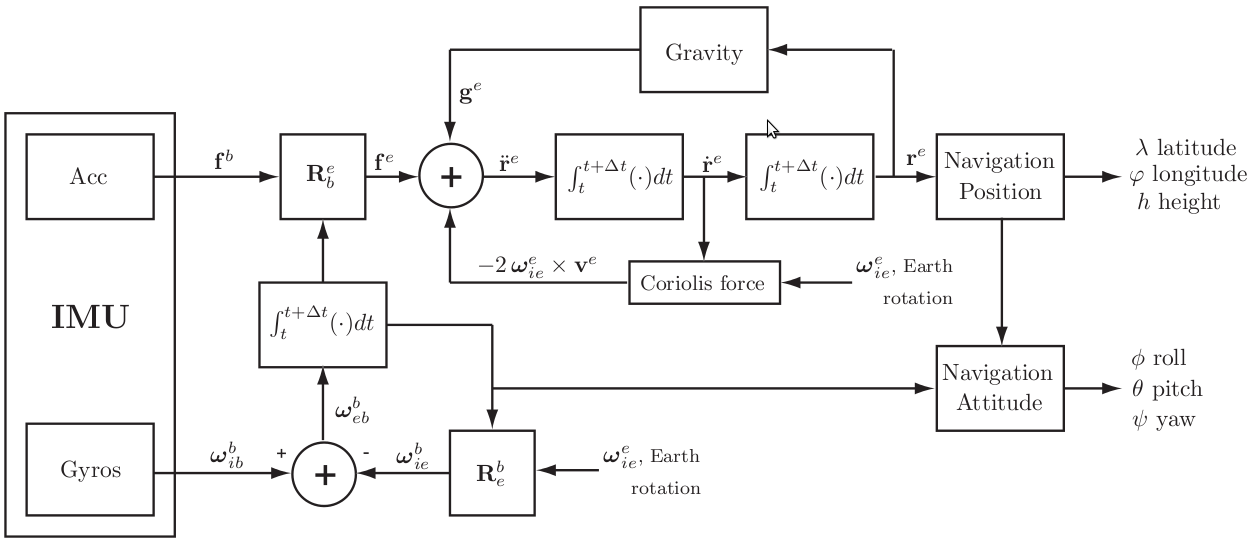
\includegraphics[scale=0.35]{sdins_algorithm}
\caption{Алгоритм роботи БІНС}
\label{fig:sdins}
\end{figure} 
Сигнали $\omega_{x,y,z}$ з виходу аналітичного компенсатора похибок використовуються 
для обчислення параметрів матриці напрямних  косинусів \textit{В}, яка визначає зв'язок 
між двома системами координат. Оскільки матриця напрямних  косинусів \textit{В} визначається 
між зв'язаними з ЛА осями й осями обертової навігаційної системи координат, то при 
розрахунках параметрів матриці \textbf{В }необхідно залучити обчислені проекції вектора 
кутової швидкості навігаційної системи координат, що відображено на схемі додатковими 
зв'язками, які враховують кутову швидкість, що виникає при обльоті сферичної Землі (
$\dot{\lambda }$, $\dot{h}$, $\dot{\varphi }$, і кутову швидкість обертання самої 
Землі $(\Omega_{\text{З}} )$.

Перетворення складових уявного прискорення $a_{x,y,z}$  від осей ЛА до осей навігаційної 
системи координат здійснюється за допомогою матриці напрямних  косинусів \textit{В}. Навігаційний 
обчислювач вирішує задачі, властиві всім платформним системам, оскільки на вході 
цього обчислювача сформовані проекції уявного прискорення на осі навігаційної системи 
координат і нічого принципово нового в розв'язанні цієї задачі немає. На виході БІНС 
формуються радіус-вектор місця розташування ЛА, вектор швидкості, а також кути орієнтації 
ЛА. 

В окремому випадку, коли за навігаційний базис вибраний горизонтальний орієнтований 
за сторонами світу тригранник, на виході системи будуть сформовані географічні (геодезичні) 
координати радіуса-вектора місця розташування $\lambda$, $\varphi$, \textit{H}, проекції 
відносної швидкості руху $V_N$, $V_E$, $V_H$, а також 
кути орієнтації ЛА в географічній системі координат -- справжній курс $\psi$, тангаж $\vartheta$ і 
крен $\gamma$. 

Обсяг обчислень у БІНС значний. Це пояснюється в основному тим фактом, що БЦОМ розв'язує 
задачі, які пов'язані з динамікою обертання ЛА, а також з динамікою поступального 
руху ЛА. Поступальні швидкості ЛА відносно малі. Наприклад, швидкість при польоті 
ЛА в напрямку на північ 1100 км/год відповідає швидкості зміни широти усього на 10 
град/год.

Таким чином, інтегрування для одержання швидкості і місця розташування можуть здійснюватися 
досить точно з використанням дуже простих методів чисельного інтегрування при низькій 
частоті повторення   в типовому випадку 10...20 Гц .

Кутові швидкості ЛА в типовому випадку за величиною на кілька порядків більші поступальних 
швидкостей. Зокрема, для маневрених ЛА кутові швидкості обертання можуть складати 
сотні градусів за секунду. В результаті цього інтегрування кутового положення в БІНС 
зв'язано з жорсткими вимогами до БЦОМ.

Оскільки для забезпечення високої точності інерціальної навігації потрібно, щоб похибки 
інтегрування кутового положення обмежувалися декількома частками кутової хвилини, 
необхідно застосовувати алгоритми інтегрування більш високого порядку при типових 
частотах повторення  80...50 Гц. 

З огляду на вище сказане, наведемо  варіант побудови алгоритмів БІНС для випадку, 
коли за навігаційний базис вибраний горизонтальний орієнтований за сторонами світу 
тригранник.
\vspace{5mm}

\textbf{Алгоритми БІНС, яка працює в географічній системі координат}

За навігаційний тригранник візьмемо тригранник \textit{NHE}, зв'язаний з земною поверхнею.
\begin{figure}[here]
\centering
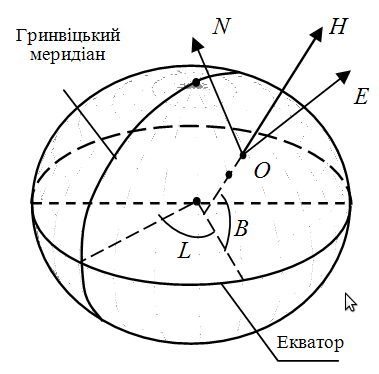
\includegraphics[scale=0.4]{earth_1}
\caption{Системи координат}
\label{fig:earth}
\end{figure} 
Виберемо наступний напрямок осей   \textit{NHE} (рис. \ref{fig:earth}):
\begin{ESKDexplanation}
\item \textit{OH} --збігається з вертикаллю;
\item \textit{ON} -- дотична до меридіана;
\item \textit{ОЕ} -- утворює праву трійку.
\end{ESKDexplanation}
В алгоритмах БІНС, зазвичай, виділяють динамічні та кінематичні рівняння. 
Динамічні рівняння реалізують трикомпонентну схему БІНС, у якій географічні координати  $\lambda$, 
$\varphi$,\textit{Н} визначаються інтегруванням рівнянь вигляду

\[\begin{array}{l} 
{\dot{\lambda}=\frac{V_{E}}{(R_{2} +H)\cos \varphi} ;} \\ 
{\dot{\varphi}=\frac{V_{N}}{R_{1} +H} ;} \\ 
{\dot{H}=V_{H,}} 
\end{array}\] 
\begin{ESKDexplanation}
\item де  $V_{N}$,$V_{E}$ -- північна та східна проекції шляхової швидкості 
(проекції на осі  системи координат \textit{NHE}  (див. рис. \ref{fig:earth}); 
\item $R_1$, \textit{R}2 -- два радіуси кривизни земного сфероїда (еліпсоїда обертання); 
\item $R_1$ -- радіус кривизни меридіонального перетину еліпсоїда (площиною \textit{HN}); 
\item $R_2$  -- радіус кривизни перетину еліпсоїда площиною \textit{HЕ} (площиною першого вертикала); 
\end{ESKDexplanation}
\[R_{1} =\frac{a(1-e^{2})}{(1-e^{2} \sin(\varphi)^{2})^{\frac{3}{2}}};\\
R_{2} =\frac{a}{\sqrt{1-e^{2} \sin(\varphi)^{2}}}.\] 
\begin{ESKDexplanation}
\item де\textit{ a}  --- велика піввісь  еліпсоїда (\textit{a }=  6378388 м); 
\item \textit{e} --- ексцентриситет еліпсоїда  ($e^{2} = 6,73 \cdot 10^{-3}$);  
\item \textit{Н}  --- висота польоту. 
\end{ESKDexplanation}
Тут можна застосовувати такі ж спрощення, що й у платформних інерціальних системах. 
Зокрема, функції   $\frac{1}{R_{1} +H}$ та $\frac{1}{R_{2} +H} $ 
з точністю до членів порядку малості $10^{-5}$ можна представити 
в наступному вигляді:

\[\begin{array}{l} 
{\frac{1}{R_{1} +H} =\frac{1}{a} [1-e^{2} -\frac{H}{a} 
-\frac{3}{2} e^{2} \sin ^{2} \varphi-2e^{2} \frac{H}{a} +3e^{2} \frac{H}{a} \sin 
^{2} \varphi + (\frac{H}{a} )^{2} +}\\
{+e^{4} (1-3\sin ^{2} B+\frac{3}{8}\sin ^{4} \varphi);} \\ 

{\frac{1}{R_{2} +H} =\frac{1}{a}[1-\frac{H}{a} 
-\frac{1}{2} e^{2} \sin ^{2} \varphi+(\frac{H}{a})^{2} +e^{2} \frac{H}{a} 
\sin ^{2} \varphi+} \\ 
{+e^{4}(\frac{1}{4} \sin ^{2} \varphi-\frac{3}{8})\sin ^{2} \varphi]} 
\end{array}\] 
Якщо у формулах $\frac{1}{R_{1} +H}$ та $\frac{1}{R_{2} +H}$ 
зберегти лише члени порядку малості $10^{-2}$ , то вони приймуть 
вигляд

\begin{equation} 
\label{eq:elips} 
\begin{array}{l} 
{\frac{1}{R_{1} +H} \approx \frac{1}{a}[1-e^{2} -\frac{H}{a} -\frac{3}{2} e^{2} \sin(B)^{2}];} \\ 
{\frac{1}{R_{2} +H} \approx \frac{1}{a}[1-\frac{H}{a} -\frac{1}{2} e^{2} \sin(\varphi)^{2}].} 
\end{array} 
\end{equation} 
Слід відзначити, що використання спрощень \eqref{eq:elips} може призвести 
до похибок, порівняних з похибками високоякісних гіроскопічних вимірників, які використовуються 
в БІНС.

Складові шляхової швидкості ЛА  $V_E$ , $V_N$ , $V_H$  одержують в результаті інтегрування 
проекцій сигналів акселерометрів, виключаючи із них  складові коріолісового прискорення  і 
прискорення сили ваги: 
\begin{equation} 
\label{eq:Vi} 
 \begin{array}{l} 
{\dot{V}_{E} =a_{E} -(V_{N} \omega_{H_{\Sigma }} -V_{H} \omega_{N_{\Sigma}} )+g_{E} ;} \\ 
{\dot{V}_{H} =a_{H} -(V_{E} \omega_{N_{\Sigma }} -V_{N} \omega_{E_{\Sigma}} )+g_{H} ;} \\ 
{\dot{V}_{N} =a_{N} -(V_{H} \omega_{E_{\Sigma }} -V_{E} \omega_{H_{\Sigma}} )+g_{N} ,} 
\end{array}
\end{equation} 
\begin{ESKDexplanation}
\item де $a_{E,H,N} $ -- проекції уявного прискорення ЛА, вимірювані акселерометрами, 
на осі навігаційного тригранника; 
\item $g_{E,H,N} $ --- проекції вектора прискорення 
сили ваги, які враховують прискорення земного тяжіння, і прискорення, що викликається 
відцентровою силою інерції і зв'язане з обертанням Землі; 
\item складові в дужках --- проекції коріолісового прискорення на осі навігаційного тригранника; 
\item $\omega_{E_{\Sigma}}$, $\omega_{H_{\Sigma}}$, $\omega_{N_{\Sigma}}$ --- проекції кутової 
швидкості навігаційного тригранника відносно інерціального простору, які враховують 
проекції кутової швидкості обертання Землі $\Omega_{E}$, $\Omega_{H}$, $\Omega_{N}$ 
і складові відносної кутової швидкості навігаційного тригранника, які обумовлені 
рухом ЛА відносно Землі $\omega_{E_{V}}$, $\omega_{H_{V}}$, $\omega_{N_{V}}$: 
\end{ESKDexplanation}
\[\omega_{N_{\Sigma }} =\omega_{N_{V}} +2\Omega_{N} ;\\ 
\omega_{H_{\Sigma }} =\omega_{H_{V}} +2\Omega_{H} ;\\
\omega_{E_{\Sigma }} =\omega_{E_{V}} +2\Omega_{E} .\] 

У свою чергу, складові відносної кутової швидкості навігаційного тригранника і швидкості 
обертання Землі визначаються співвідношеннями
\[\begin{array}{l} 
{\omega_{E_{V}} =-\frac{V_{N}}{R_{1} +H} =-\dot{\varphi};} \\ 
{\omega_{H_{V}} =\frac{V_{E}}{(R_{2} +H)} tg\varphi=\dot{\lambda}\sin \varphi;} \\ 
{\omega_{N_{V}} =\frac{V_{E}}{(R_{2} +H)} =\dot{\lambda}\cos \varphi;} \end{array}\] 

\[\Omega_{N} =\Omega_{\text{З}}\cos \varphi;
\Omega_{H} =\Omega_{\text{З}}\sin \varphi; 
\Omega_{E} =0,\] 

\begin{ESKDexplanation}
 \item де  $\Omega_{\text{З}} $ --- кутова швидкість обертання Землі ($\Omega_{\text{З}}=7,27 \cdot 10^{-5}$ рад/с).
\end{ESKDexplanation}

Детермінована математична модель прискорення сили ваги існує тільки для нормальної 
складової поля сили ваги, що відповідає земному еліпсоїду з рівномірним розподілом 
мас в об'ємі цієї фігури. Градієнт цього поля в будь-якій точці, що належить поверхні 
еліпсоїда, спрямований за нормаллю до неї і розташований у площині меридіонального 
перетину. Оскільки точка місцеположення ЛА не належить поверхні Землі, то вектор 
градієнта нормального поля сили ваги $\bar{g}$ в цій точці не буде спрямований за 
лінією нормалі, опущеної з неї до поверхні земного еліпсоїда (вісь \textit{ОН}). 
Разом з тим, цей вектор буде розташований у площині меридіана точки \textit{О}, тобто 
в площині \textit{NOH}. Тоді, використовуючи  потенційну функцію нормального поля 
тяжіння земного сфероїда, з точністю до членів порядку малості $10^{-5}$  співвідношення 
для проекцій складових поля сили ваги $\bar{g}$ мають такий вигляд:
\[\begin{array}{l} 
{g_{E} =0;} \\
{g_{N} =\frac{1}{2} g[\frac{H}{a} (e^{2} -5q)+qe^{2} \sin^{2}\varphi]\sin^2\varphi;}\\
{g_{H} =-g\left\{1-2\frac{H}{a} -\right. (e^{2} +2q-3\frac{H}{a})
\frac{H}{a} +\left[\frac{1}{2} (5q-e\right. ^{2} )-\frac{1}{8} e^{4} +\frac{17}{18}qe^{2} +} \\ 
{ +(3e^{2} - 5q)\frac{H}{a} ]\sin ^{2} B-\frac{1}{2} qe^{2} \sin ^{4} \varphi+\frac{1}{16} e^{2} 
(\frac{1}{2} e^{2} -7q)\sin ^{2} 2\varphi\},} 
\end{array}\]
\begin{ESKDexplanation}
\item де $g= 9,78049 \text{м}/\text{с}^{2}$ прискорення сили ваги на екваторі; 
\item \textit{q} = $\Omega_{\text{З}}^{2} $ \textit{a/g} = 0,00346775 --- відношення 
відцентрової сили, обумовленої обертанням Землі, до сили ваги на екваторі. 
\end{ESKDexplanation}

З точністю до величин порядку малості $10^{-4}$ співвідношення для проекцій складових 
поля сили ваги $\bar{g}$ декілька спрощуються:

\[\begin{array}{l} 
{ g_{E} =0;} \\ 
{g_{N} =g\sin 2\varphi+\frac{5}{2} q\sin ^{2} B\frac{H}{a}(\frac{e^{2}}{2} -2q);} \\ 
{g_{H} =-g\left[1-\frac{e^{2}}{2}\sin ^{2} \varphi+\frac{3}{2} q\sin ^{2} \varphi+e^{4}(-\frac{1}{8} \sin ^{2} \varphi+\frac{1}{32} 
\sin ^{2} 2\varphi\right)+} \\ 
{ +e^{2} q\left(-\frac{17}{28} 
\sin ^{2} \varphi-\frac{5}{16} \sin ^{2} 2\varphi\right)+\frac{H}{a} e^{2} (3\sin ^{2} \varphi-1)+}\\ 
{ +\frac{Hq}{a} (-1-6\sin ^{2}\varphi)-2\frac{H}{a} +3\frac{H^{2}}{a^{2}}],} 
\end{array}\] 

а при малих значеннях висоти ($Н\leq$ 100 км ) проекції вектора  $\bar{g}$ на 
осі \textit{NHE}, якщо в них зберегти лише члени порядку малості $10^{-2}$, 
взагалі мають простий вигляд: 
\[\begin{array}{l} 
{g_{E} =0;}\\
{g_{N} =0;}\\ 
{g_{H} =-g(1+5,2884\cdot 10^{-3} \sin ^{2}\varphi)[1-\frac{2H}{a}
(1-e\sin^{2}\varphi )]} 
\end{array}\] 
Є й інші форми запису даної складової.

При розв'язанні кінематичних рівнянь розраховуються проекції $a_{E,H,N} $ уявного 
прискорення ЛА на осі навігаційного тригранника \textit{NHE}за показаннями акселерометрів 
зі зв'язаної з ЛА системи координат \textit{XYZ} з використанням матриці напрямних  
косинусів \textbf{В}
\[ \left[\begin{array}{c} 
{a_{N}} \\ 
{a_{H}} \\ 
{a_{E}}
\end{array}\right]=B
\left[\begin{array}{c} 
{a_{x_{\text{ЛА}}}} \\ 
{a_{y_{\text{ЛА}}}} \\ 
{a_{z_{\text{ЛА}}}} 
\end{array}\right]\] 
Матриця напрямних  косинусів  має такий вигляд:
\[B=\left[\begin{array}{c|c|c} 
{\cos \psi \cos \vartheta } & 
{\sin \psi \sin \gamma -\cos \psi \sin \vartheta \cos \gamma } & 
{\sin \psi \cos \gamma +\sin \gamma \sin \vartheta \cos \psi } \\  \hline {\sin \vartheta } & 
{\cos \vartheta \cos \gamma} & 
{-\cos \vartheta \sin \gamma } \\  \hline {-\sin \psi \cos \vartheta } & 
{\cos \psi \sin \gamma +\sin \psi \sin \vartheta \cos \gamma } & 
{\cos \psi \cos \gamma -\sin \psi \sin \vartheta \sin \gamma } 
\end{array}\right]\] 
\begin{ESKDexplanation}
\item де $\gamma$, $\vartheta$, $\psi$ -- кути крену, тангажа і рискання. Кут рискання 
відрізняється від географічного курсу $\psi$г знаком, тобто $\psi$г = $\psi$.
\end{ESKDexplanation}
Матриця напрямних  косинусів \textbf{В} може бути отримана в різні способи. Наведемо приклади 
деяких з них. 

Знайти матрицю \textbf{В} можна в результаті розв'язання 
узагальненого рівняння Пуассона за інформацією про кутову швидкість ЛА відносно інерціального 
простору $\omega_{\text{ЛА}}$ і кутову швидкість навігаційної системи координат відносно 
інерціального простору $\omega_{NHE}$, яка враховує кутову швидкість 
обертання Землі і кутову швидкість, обумовлену обльотом ЛА сферичної Землі 
\[  \dot{B}=B\omega_{\text{ЛА}} -\omega_{NHE}B\] 
де 
\[\omega_{\text{ЛА}} =\left[\begin{array}{ccc} 
{0} & {-\omega_{z_{\text{ЛА}}}} & {\omega_{y_{\text{ЛА}}}} \\ 
{\omega_{z_{\text{ЛА}}}} & {0} & {-\omega_{x_{\text{ЛА}}}} \\ 
{-\omega_{y_{\text{ЛА}}}} & {\omega_{x_{\text{ЛА}}}} & {0} 
\end{array}\right];\]\\
\[\omega_{NHE} =\left[\begin{array}{ccc} 
{0} & {-(\omega_{E_{V}} +\Omega_{E} )} & {(\omega_{H_{V}} +\Omega_{H} )} \\ 
{(\omega_{E_{V}} +\Omega_{E})} & {0} & {-(\omega_{N_{V}} +\Omega_{N} )} \\ 
{-(\omega_{H_{V}} +\Omega_{H})}& {(\omega_{N_{V}} +\Omega_{N} )} & {0} 
\end{array}\right];\] 
\begin{ESKDexplanation}
  \item $\omega_{x_{\text{ЛА}}}$, $\omega_{y_{\text{ЛА}}}$, $\omega_{z_{\text{ЛА}}}$  -- кутові 
  швидкості ЛА відносно зв'язаних осей, вимірювані датчиками кутової швидкості; 
  \item $\omega_{E_{V}}$, $\omega_{H_{V}}$, $\omega_{N_{V}}$ були визначені раніше.
\end{ESKDexplanation}
За елементами матриці  \textit{B} визначаються кути орієнтації ЛА: крен $\gamma$, тангаж 
$\vartheta$ рискання (курс) $\psi $: 
\begin{equation} 
\label{eq:angels} 
\begin{array}{l} 
{\gamma ={\rm arctg}\left(
\frac{-b_{23}}{b_{22}} \right)={\rm arcsin}\left(\frac{-b_{23}}{\sqrt{1-b_{21}^{2} 
}} \right)={\rm arccos}\left(\frac{b_{22}}{\sqrt{1-b_{21}^{2}}} \right)\; ; } \\ 
{\vartheta ={\rm arctg}\left(\frac{b_{21}}{\sqrt{b_{22}^{2} +b_{33}^{2}}} 
\right){\rm \; }={\rm arcsin(}b_{21} {\rm )}={\rm arccos}\left(\sqrt{1-b_{21}^{2} 
} \right)} \\ 
{\psi =-{\rm arctg}\left(\frac{b_{31}}{b_{11}} \right)={
\rm arcsin}\left(\frac{-b_{31}}{\sqrt{1-b_{21}^{2}}} \right)={\rm arccos}\left(
\frac{b_{11}}{\sqrt{1-b_{21}^{2}}} \right).} 
\end{array} 
\end{equation} 
Інший алгоритм отримання матриці напрямних косинусів припускає її  формування безпосередньо 
за кутами  $\gamma$, $\vartheta$, $\psi$. 
\begin{figure}[here]
\centering
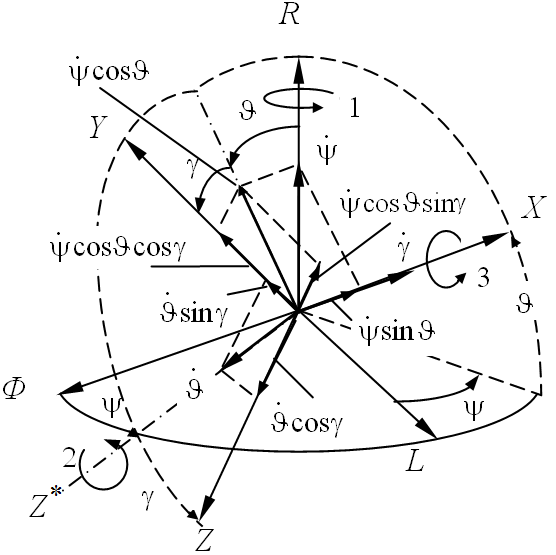
\includegraphics[scale=0.4]{dcm_other_meth}
\caption{Кінематичні співвідношення між кутами}
\label{fig:kinemat}
\end{figure} 
Кінематичні співвідношення між кутами $\gamma$, $\vartheta$, $\psi$ і проекціями вектора абсолютної кутової 
швидкості на осі зв'язаної системи координат $\omega_{x_{\Sigma }}$ , $\omega_{y_{\Sigma }}$, 
$\omega_{z_{\Sigma}} $ можна одержати з рис. \ref{fig:kinemat}, 
на якому показано перетворення навігаційної системи координат \textit{OLR$\Phi $ }у 
зв'язану \textit{OXYZ} шляхом трьох поворотів: \textit{1}   навколо осі \textit{OR}; \textit{2}  
навколо проміжної осі \textit{OZ*}; \textit{3}  навколо осі \textit{OX}.

 Звичайно, що кутові швидкості $\dot{\psi }$, $\dot{\vartheta }$, $\dot{\gamma }$, 
які спрямовані уздовж відповідних осей, є складовими абсолютної кутової швидкості 
ЛА.

 Проектуючи $\dot{\psi }$,$\dot{\vartheta }$, $\dot{\gamma }$на осі зв'язаної системи 
координат, отримаємо:

\[\begin{array}{l} 
{\omega_{x_{\Sigma }} =\dot{\gamma }+\dot{\psi }\sin \vartheta ;} \\ 
{\omega_{y_{\Sigma }} =\dot{\vartheta }\sin \gamma +\dot{\psi}\cos \vartheta\cos \gamma ;} \\ 
{\omega_{z_{\Sigma }} =\dot{\vartheta }\cos \gamma -\dot{\psi}\cos \vartheta \sin \gamma .} 
\end{array}\] 
Розв'язуючи ці співвідношення, одержимо такі кінематичні рівняння:
\[\begin{array}{l} 
{\dot{\psi }=(\omega_{y_{\Sigma }} \cos \gamma -\omega_{z_{\Sigma }} \sin \gamma)\sec \vartheta ;} \\ 
{\dot{\gamma }=\omega_{x_{\Sigma }} +tg\vartheta (\omega_{z_{\Sigma }} \sin \gamma -\omega_{y_{\Sigma }} \cos \gamma );} \\ 
{\dot{\vartheta }=\omega_{y_{\Sigma }} \sin \gamma +\omega_{z_{\Sigma }} \cos \gamma.} 
\end{array}\] 
У свою чергу 
\[ \begin{array}{l} 
  {\omega_{y_{\Sigma }} =\omega_{y_{\text{ЛА}}} -\omega_{y_{_{NHE}}};} \\ 
  {\omega_{x_{\Sigma }} =\omega_{x_{\text{ЛА}}}  -\omega_{x_{NHE}} ;} \\ 
  {\omega_{z_{\Sigma }} =\omega_{z_{\text{ЛА}}}  -\omega_{z_{NHE}}.} \end{array}\] 
\begin{ESKDexplanation}
\item де $\omega_{y_{\text{ЛА}}}$,$\omega_{x_{\text{ЛА}}}$,$\omega_{z_{\text{ЛА}}}$ -- проекції 
кутової швидкості ЛА відносно інерціального простору на осі зв'язаної системи координат, 
вимірювані датчиками кутових швидкостей;
\item $\omega_{y_{_{NHE}}}$,$\omega_{x_{_{NHE}}}$,$\omega_{z_{_{NHE}}}$  -- проекції кутової швидкості навігаційного тригранника 
відносно інерціального простору на осі зв'язаної системи координат, які враховують 
проекції кутової швидкості обертання Землі  $\Omega_{H}$,$\Omega_{E}$ ,$\Omega_{N}$
і складові відносної кутової швидкості навігаційного тригранника, 
що обумовлені рухом ЛА відносно Землі $\omega_{H_{V}}$ , $\omega_{E_{V}}$ ,
$\omega_{N_{V}} $. 
\end{ESKDexplanation}
% \includegraphics[bb=0mm 0mm 208mm 296mm, width=36.3mm, height=6.6mm, viewport=3mm 
% 4mm 205mm 292mm]{image1.eps} 
Ці проекції кутової швидкості визначаються в результаті 
розв'язання матричного рівняння 
\[\left
[\begin{array}{c} {\omega_{x_{NHE}}} \\ 
{\omega_{y_{NHE}}} \\ 
{\omega_{z_{NHE}}} 
\end{array}\right]
=B^{T} 
\left[\begin{array}{c} {\omega_{N_{V} 
} +\Omega_{N}} \\ 
{\omega_{H_{V}} +\Omega_{H}} \\ 
{\omega_{E_{V}} +\Omega_{E}} 
\end{array}\right] .\] 
Перевагою такого підходу до визначення кутів орієнтації ЛА (інтегруванням диференціальних 
рівнянь, що описують швидкості зміни кутів Ейлера, а не за арктангенсами відношення 
елементів матриці напрямних  косинусів) є відсутність обмежень $\gamma$ $\pm90^{o}$, 
що особливо важливо при визначенні курсу ЛА на віражах. 

Тривимірні матриці напрямних  косинусів досить зручні для обчислень у бортовій ЦОМ. 
Однак формування матриці \textbf{В} з використанням тригонометричних функцій вимагає 
значних обчислювальних витрат. 

Для визначення орієнтації ЛА можна використовувати не тільки напрямні косинуси, але 
і параметри Родрига-Гамільтона у формі кватерніонів. Достоїнство методу кватерніонів 
полягає в тому, що він дозволяє описувати перехід від однієї системи координат до 
іншої за допомогою всього лише чотирьох чисел, а не 9 напрямних  косинусів.

Кватерніонний метод ґрунтується  на теоремі Ейлера, яка доводить, що будь-який поворот 
однієї системи координат відносно іншої можна подати, як поворот на деякий кут навколо 
однієї нерухомої осі.

Кватерніон є компактною формою запису орієнтації зазначеної осі (векторна частина 
кватерніона $\lambda_{1} ,\lambda_{2} ,\lambda_{3} $) і кута повороту (скалярна 
частина кватерніона $\lambda_{0} $) відповідно до теореми Ейлера.

Застосування кватерніонів дозволяє подати ортогональні перетворення у формі множення 
кватерніонів. Дії над кватерніонами допускають матричні операції з використанням 
симетризованих матриць, що дуже зручно при створенні програм бортових обчислювачів. 

Відповідно 
до теореми Ейлера-Шаля усяке переміщення твердого тіла, яке має нерухому точку, можна 
зобразити як результат повороту навколо незмінного напрямку (ейлерової осі) на певний 
кут $\varphi $. Якщо зв'язати з розглянутим твердим тілом правий ортогональний координатний 
тригранник, то параметри Родрига-Гамільтона $\lambda_{0}$ ,$\lambda_{1}$, $\lambda_{2}$,
$\lambda_{3}$ ,що однозначно характеризують згадані переміщення, можна задати 
такими виразами: 
\[\lambda_{1} =\frac{l_{1} \sin \varphi }{2};
  \lambda_{2} =\frac{l_{2} \sin \varphi }{2};
  \lambda_{3} =\frac{l_{3} \sin \varphi }{2};
  \lambda_{0} =\frac{\cos \varphi }{2} ,\] 
\begin{ESKDexplanation}
 \item де $l_{1} ,l_{2} ,l_{3} -$косинуси кутів, утворених ейлеровою віссю з осями тригранника 
в його вихідному та кінцевому положенні. 
\end{ESKDexplanation}

Зв'яжемо з ЛА, на якому встановлена БІНС, ортонормований базис \textbf{Е} -- 
праву трійку взаємно ортогональних одиничних 
векторів $e_{1}$ ,$e_{2}$ ,$e_{3}$. Орієнтацію базису \textbf{Е} відносно ортонормованого 
інерціального базису \textbf{І}, складеного з ортів $i_{1}$ ,$i_{2}$ ,$i_{3}$ , охарактеризуємо 
параметрами Родрига-Гамільтона $\lambda_{0}$ ,$\lambda_{1}$ ,$\lambda_{2}$ ,$\lambda 
_{3}$. Матриця напрямних  косинусів, що обчислена за параметрами Родрига-Гамільтона 
(кватерніонами), має такий вигляд:

\[B=\left[
\begin{array}{ccc} {1-2(\lambda_{2}^{2} +\lambda_{3}^{2} )} & 
{2(\lambda_{1} \lambda_{2} -\lambda_{0} \lambda_{3} )} & 
{2(\lambda_{1} \lambda_{3} +\lambda_{0} \lambda_{2} )} \\ 
{2(\lambda_{1} \lambda_{2} +\lambda_{0} \lambda_{3} )} & 
{1-2(\lambda_{1}^{2} +\lambda_{3}^{2} )} & 
{2(\lambda_{2} \lambda_{3} -\lambda_{0} \lambda_{1} )} \\ 
{2(\lambda_{1} \lambda_{3} -\lambda_{0} \lambda_{2} )} & 
{2(\lambda_{2} \lambda_{3} +\lambda_{0} \lambda_{1} )} & 
{1-2(\lambda_{1}^{2} +\lambda_{2}^{2} )} \end{array}\right].\] 

Вимірники кутової швидкості, що входять до складу БІНС, вимірюють координати 
$\omega_{x}$, $\omega_{y}$, $\omega_{z}$ вектора $\bar{\Omega }$ абсолютної кутової швидкості 
базису \textbf{Е}, що задані в цьому базисі. Необхідно, знаючи значення параметрів 
Родрига-Гамільтона в момент часу $t=t_{0} $ і використовуючи сигнали вимірників кутової 
швидкості, обчислювати параметри Родрига-Гамільтона при $t>t_{0} $. У початковий 
момент часу за інформацією про кути крену тангажа і курсу можна розрахувати вихідні 
значення параметрів Родрига-Гамільтона: 
\[\begin{array}{l} 
{\lambda_{0_{0}} =\sin  \left({\gamma_{0}  \mathord{
\left/{\vphantom{\gamma_{0}  2}}\right.\kern-\nulldelimiterspace} 2} \right)\sin 
 \left({\vartheta_{0}  \mathord{\left/{\vphantom{\vartheta_{0}  2}}\right.\kern-
\nulldelimiterspace} 2} \right)\sin  \left({\psi_{0}  \mathord{\left/{\vphantom{
\psi_{0}  2}}\right.\kern-\nulldelimiterspace} 2} \right)+\cos  \left({\gamma 
_{0}  \mathord{\left/{\vphantom{\gamma_{0}  2}}\right.\kern-\nulldelimiterspace} 
2} \right)\cos  \left({\vartheta_{0}  \mathord{\left/{\vphantom{\vartheta_{0}  
2}}\right.\kern-\nulldelimiterspace} 2} \right)\cos  \left({\psi_{0}  \mathord{
\left/{\vphantom{\psi_{0}  2}}\right.\kern-\nulldelimiterspace} 2} \right);} \\ 

{\lambda_{1_{0}} =-\sin  \left({\vartheta_{0}  \mathord{\left/{\vphantom{
\vartheta_{0}  2}}\right.\kern-\nulldelimiterspace} 2} \right)\sin  \left({\psi 
_{0}  \mathord{\left/{\vphantom{\psi_{0}  2}}\right.\kern-\nulldelimiterspace} 2} 
\right)\cos  \left({\gamma_{0}  \mathord{\left/{\vphantom{\gamma_{0}  2}}\right.
\kern-\nulldelimiterspace} 2} \right)+\sin \left({\gamma_{0}  \mathord{\left/{\vphantom{
\gamma_{0}  2}}\right.\kern-\nulldelimiterspace} 2} \right)\cos  \left({\vartheta 
_{0}  \mathord{\left/{\vphantom{\vartheta_{0}  2}}\right.\kern-\nulldelimiterspace} 
2} \right)\cos  \left({\psi_{0}  \mathord{\left/{\vphantom{\psi_{0}  2}}\right.
\kern-\nulldelimiterspace} 2} \right);} \\ 

{\lambda_{2_{0}} =\sin \left({
\gamma_{0}  \mathord{\left/{\vphantom{\gamma_{0}  2}}\right.\kern-\nulldelimiterspace} 
2} \right)\cos  \left({\vartheta_{0}  \mathord{\left/{\vphantom{\vartheta_{0}  
2}}\right.\kern-\nulldelimiterspace} 2} \right)\sin  \left({\psi_{0}  \mathord{
\left/{\vphantom{\psi_{0}  2}}\right.\kern-\nulldelimiterspace} 2} \right)+\sin 
 \left({\vartheta_{0}  \mathord{\left/{\vphantom{\vartheta_{0}  2}}\right.\kern-
\nulldelimiterspace} 2} \right)\cos  \left({\gamma_{0}  \mathord{\left/{\vphantom{
\gamma_{0}  2}}\right.\kern-\nulldelimiterspace} 2} \right)\cos  \left({\psi_{0}  
\mathord{\left/{\vphantom{\psi_{0}  2}}\right.\kern-\nulldelimiterspace} 2} \right);}\\ 

{\lambda_{3_{0}} =\sin  \left({\psi_{0}  \mathord{\left/{\vphantom{
\psi_{0}  2}}\right.\kern-\nulldelimiterspace} 2} \right)\cos  \left({\gamma_{0}  
\mathord{\left/{\vphantom{\gamma_{0}  2}}\right.\kern-\nulldelimiterspace} 2} \right)
\cos  \left({\vartheta_{0}  \mathord{\left/{\vphantom{\vartheta_{0}  2}}\right.
\kern-\nulldelimiterspace} 2} \right)-\sin  \left({\gamma_{0}  \mathord{\left/{
\vphantom{\gamma_{0}  2}}\right.\kern-\nulldelimiterspace} 2} \right)\sin  \left({
\vartheta_{0}  \mathord{\left/{\vphantom{\vartheta_{0}  2}}\right.\kern-\nulldelimiterspace} 
2} \right)\cos  \left({\psi_{0}  \mathord{\left/{\vphantom{\psi_{0}  2}}\right.
\kern-\nulldelimiterspace} 2} \right).} \end{array}\] 

Поточні значення параметрів $\lambda_{0}$ ,$\lambda_{1}$ ,$\lambda_{2}$ ,$\lambda_{3}$ можна 
визначити, знаючи проекції кутової швидкості ЛА $\omega_{x}$ ,$\omega_{y}$ ,$\omega_{z}$ 
на зв'язаній осі $XYZ$, шляхом розв'язання лінійного диференціального рівняння 
зі змінними коефіцієнтами. У цьому випадку параметри $\lambda_{0}$ ,$\lambda_{1}$ 
,$\lambda_{2}$ ,$\lambda_{3}$ кватерніона  описують  положення  осей ЛА  $XYZ$  відносно  
інерціального простору:

\[\dot{\lambda }=\frac{1}{2} \Omega(t)\cdot \lambda(t)\] 
\begin{ESKDexplanation}
\item де $\Omega(t)$ -- кососиметрична $(4\times 4)$-матриця, яка 
відповідає вектору $\omega =[\omega_{x} \omega_{y} \omega_{z}]^{T}  $
\end{ESKDexplanation}
\[\Omega (t)=\left[
\begin{array}{cccc} 
  {0} & {-\omega_{x}} & {-\omega_{y}} & {-\omega_{z}} \\ 
  {\omega_{x}} & {0} & {\omega_{z}} & {-\omega_{y}} \\ 
  {\omega_{y}} & {-\omega_{z}} & {0} & {\omega_{x}} \\ 
  {\omega_{z}} & {\omega_{y}} & {-\omega_{x}} & {0} 
\end{array}\right];
\lambda =\left[\begin{array}{c} 
  {\lambda_{0}} \\ 
  {\lambda_{1}} \\ 
  {\lambda_{2}} \\ 
  {\lambda_{3}} 
\end{array}
\right].\] 

Цей вираз є кватерніонним однорідним лінійним диференціальним рівнянням першого порядку 
зі змінним коефіцієнтом у вигляді гіперкомплексного числа з дійсною частиною, що 
дорівнює нулю. У скалярній формі це рівняння  має такий вигляд:

\[\begin{array}{l} 
{\dot{\lambda}_{0} =-0,5(\omega_{x} \lambda_{1} +\omega_{y} \lambda_{2} +\omega_{z} \lambda_{3} ;} \\ 
{\dot{\lambda}_{1} =-0,5(\omega_{x} \lambda_{0} +\omega_{z} \lambda_{2} +\omega_{y} \lambda_{3});} \\ 
{\dot{\lambda}_{2} =-0,5(\omega_{y} \lambda_{0} +\omega_{z} \lambda_{1} +\omega_{x} \lambda_{3});} \\ 
{\dot{\lambda}_{3} =-0,5(\omega_{z} \lambda_{0} +\omega_{y} \lambda_{1} +\omega_{x} \lambda_{2}).}
\end{array}\] 

Динаміка зміни параметрів кватерніона у випадку, коли кватерніон характеризує взаємне 
положення зв'язаних з ЛА осей $XYZ$ і обертових навігаційних осей \textit{NHE}, описується 
рівняннями
\begin{equation}
 \left[\begin{array}{c} 
{\dot{\lambda }_{0}} \\ 
{\dot{\lambda }_{1}} \\ 
{\dot{\lambda }_{2}} \\ 
{\dot{\lambda }_{3}} 
\end{array}\right]=\frac{1}{2} \left[\begin{array}{cccc}
{0} & {-\omega_{x\Sigma }} & {-\omega_{y\Sigma }} & {-\omega_{z\Sigma }} \\ 
{\omega_{x\Sigma }} & {0} & {\omega_{z\Sigma }} & {-\omega_{y\Sigma }} \\ 
{\omega_{y\Sigma }} & {-\omega_{z\Sigma }} & {0} & {\omega_{x\Sigma }} \\ 
{\omega_{z\Sigma }} & {\omega_{y\Sigma }} & {-\omega_{x\Sigma }} & {0} 
\end{array}
\right]\cdot 
\left[\begin{array}{c} 
{\lambda_{0}} \\ {\lambda_{1}} \\ {\lambda_{2}} \\ {\lambda_{3}} 
\end{array}\right] 
\label{eq:qdiff}
\end{equation}

\begin{ESKDexplanation}
 \item У свою чергу  

\[\omega_{x_{\Sigma }} =\omega_{x_{\text{ЛА}}} -\omega_{x_{NHE}} ;  \omega 
_{y_{\Sigma }} =\omega_{y_{\text{ЛА}}} -\omega_{y_{NHE}} ;  \omega_{z_{\Sigma 
}} =\omega_{z_{\text{ЛА}}} -\omega_{z_{NHE}} ,\] 

де  $\omega_{y_{\text{ЛА}}}$, $\omega_{x_{\text{ЛА}}}$, $\omega_{z_{\text{ЛА}}}$ --
проекції кутової швидкості ЛА відносно інерціального простору на осі 
зв'язаної системи координат, вимірювані датчиками кутових швидкостей;

 \item $\omega_{x_{NHE}} ,\omega_{y_{NHE}} ,\omega_{z_{NHE}} $ -- проекції кутової 
швидкості навігаційної системи координат відносно інерціального простору на осі зв'язаної 
системи координат, що визначаються в результаті розв'язання матричного рівняння 
\[\left[
\begin{array}{c} 
{\omega_{x_{NHE}}} \\ 
{\omega_{y_{NHE}}} \\ 
{\omega_{z_{NHE}}} 
\end{array}\right]=B^{T} 
\left[\begin{array}{c} 
{\omega_{N_{V}} +\Omega_{N}} \\ 
{\omega_{H_{V}} +\Omega_{H}} \\ 
{\omega_{E_{V}} +\Omega_{E}} 
\end{array}\right].\] 
\end{ESKDexplanation}
Ці складові розраховуються й у раніше розглянутих алгоритмах.


У скалярній формі рівняння \eqref{eq:qdiff} мають вигляд:
\[\begin{array}{l} 
{\dot{\lambda }_{0} =-0,5(\omega_{x\Sigma } \lambda_{1} +\omega_{y\Sigma } \lambda_{2} +\omega_{z\Sigma } \lambda_{3} );} \\ 
{\dot{\lambda }_{1} =-0,5(\omega_{x\Sigma } \lambda_{0} +\omega_{z\Sigma } \lambda_{2} +\omega_{y\Sigma } \lambda_{3} );} \\ 
{\dot{\lambda }_{2} =-0,5(\omega_{y\Sigma } \lambda_{0} +\omega_{z\Sigma } \lambda_{1} +\omega_{x\Sigma } \lambda_{3} );} \\ 
{\dot{\lambda }_{3} =-0,5(\omega_{z\Sigma } \lambda_{0} +\omega_{y\Sigma } \lambda_{1} +\omega_{x\Sigma } \lambda_{2} ).} 
\end{array}\] 
Матрицю \textit{В} перерахування зі зв'язаної в географічну систему координат можна 
також отримати шляхом перемножування двох матриць, з яких одна перераховує зі зв'язаних 
у інерціальні осі, друга -- з інерціальних у географічні. Кожна з двох матриць також 
обчислюється на основі параметрів Родрига-Гамільтона, які у свою чергу визначаються 
чисельним алгоритмом другого порядку, побудованим на основі методу послідовних наближень  
Пікара:
\[B=C^{T}A\]

\[A=\left[ \begin{array}{ccc} 
{1-2(\lambda_{2}^{2} +\lambda_{3}^{2} )} & {2(\lambda_{1} \lambda_{2}-\lambda_{0} \lambda_{3})} & {2(\lambda_{1} \lambda_{3} +\lambda_{0}\lambda_{2} )} \\ 
{2(\lambda_{1} \lambda_{2} +\lambda_{0} \lambda_{3} )} & {1-2(\lambda_{1}^{2} +\lambda_{3}^{2} )} & {2(\lambda_{2} \lambda_{3} -\lambda_{0}\lambda_{1})} \\ 
{2(\lambda_{1} \lambda_{3} -\lambda_{0} \lambda_{2} )} & {2(\lambda_{2} \lambda_{3} +\lambda_{0} \lambda_{1} )} & {1-2(\lambda_{1}^{2} +\lambda_{2}^{2})} 
\end{array}  \right];\]


\begin{equation}
\label{eq:qcalc} 
\begin{array}{cccc} 
{\lambda_{0}^{(k+1)}=\lambda_{0}^{(k)} -\lambda_{0}^{(k)} {e \mathord{/{\vphantom{e 8}}.\kern-\nulldelimiterspace} 8} 
-0,5(\lambda_{1}^{(k)} \Delta \beta_{x} +\lambda_{2}^{(k)} \Delta \beta_{y} +\lambda_{3}^{(k)} \Delta \beta_{z});}\\ 
{\lambda_{1}^{(k+1)} =\lambda_{1}^{(k)} -\lambda_{1}^{(k)} {e \mathord{/{\vphantom{e 8}}.\kern-\nulldelimiterspace} 8}
-0,5(\lambda_{0}^{(k)}\Delta \beta_{x} +\lambda_{3}^{(k)} \Delta \beta_{y} +\lambda_{2}^{(k)} \Delta\beta_{z});} \\ 
{\lambda_{2}^{(k+1)} =\lambda_{2}^{(k)} -\lambda_{2}^{(k)} {e \mathord{/{\vphantom{e 8}}.\kern-\nulldelimiterspace} 8} 
-0,5(\lambda_{3}^{(k)} \Delta \beta_{x} +\lambda_{0}^{(k)} \Delta \beta_{y}+\lambda_{1}^{(k)} \Delta \beta_{z} )  ;} \\ 
{\lambda_{3}^{(k+1)} =\lambda_{3}^{(k)} -\lambda_{3}^{(k)} {e \mathord{/{\vphantom{e 8}}.\kern-\nulldelimiterspace} 8} 
-0,5(\lambda_{2}^{(k)} \Delta \beta_{x} +\lambda_{1}^{(k)} \Delta \beta_{y} +\lambda_{0}^{(k)} \Delta \beta_{z} )  ,} 
\end{array} 
\end{equation}

\begin{ESKDexplanation}
\item де   $e=\Delta \beta_{x}^{2} +\Delta \beta_{y}^{2} +\Delta \beta_{z}^{2} ;$
\[\Delta \beta_{x} =\int_{t_{k}}^{t_{k} +1}\omega_{x_{\text{ЛА}}} dt ;   
 \Delta \beta_{y} =\int_{t_{k}}^{t_{k} +1}\omega_{y_{\text{ЛА}}} dt ;   
 \Delta \beta_{z} =\int_{t_{k}}^{t_{k} +1}\omega_{z_{\text{ЛА}}} dt ;\] 

\item $\Delta $$\beta $\textit{x}, $\Delta $$\beta $\textit{y}, $\Delta $$\beta $\textit{z }-- збільшення 
інтегралів від проекцій абсолютної кутової швидкості ЛА на осі чутливості гіроскопів 
(показання датчиків кутової швидкості БІНС, які вимірюють не проекції кутових швидкостей, 
а збільшення кутів повороту навколо своїх осей чутливості, тобто показання інтегруючих 
датчиків кутової швидкості):
\end{ESKDexplanation}
\[C=\left[\begin{array}{ccc} 
{1-2(\mu_{2}^{2} +\mu_{3}^{2} )} & {2(\mu_{1} \mu_{2} -\mu_{0} \mu_{3} )} & {2(\mu_{1} \mu_{3} +\mu_{0} \mu_{2} )} \\ 
{2(\mu_{1} \mu_{2} +\mu_{0} \mu_{3} )} & {1-2(\mu_{1}^{2} +\mu_{3}^{2} )} & {2(\mu_{2} \mu_{3} -\mu_{0} \mu_{1} )} \\ 
{2(\mu_{1} \mu_{3} -\mu_{0} \mu_{2} )} & {2(\mu_{2} \mu_{3} +\mu_{0} \mu_{1} )} & {1-2(\mu_{1}^{2} +\mu_{2}^{2} )} 
\end{array}  \right];\] 

\[\begin{array}{l} 
{\mu_{0}^{(k+1)}=\mu_{0}^{(k)} -0,5\left(\mu_{1}^{(k)} \Omega_{x} +\mu_{2}^{(k)} \Omega_{y}+\mu_{3}^{(k)} \Omega_{z} \right) dt;}\\ 
{\mu_{1}^{(k+1)}=\mu_{1}^{(k)} -0,5\left(\mu_{0}^{(k)} \Omega_{x} +\mu_{3}^{(k)} \Omega_{y}+\mu_{2}^{(k)} \Omega_{z} \right) dt;} \\ 
{\mu_{2}^{(k+1)}=\mu_{2}^{(k)} -0,5\left(\mu_{3}^{(k)} \Omega_{x} +\mu_{0}^{(k)} \Omega_{y}+\mu_{1}^{(k)} \Omega_{z} \right) dt;} \\ 
{\mu_{3}^{(k+1)}=\mu_{3}^{(k)} -0,5\left(\mu_{2}^{(k)} \Omega_{x} +\mu_{1}^{(k)} \Omega_{y} +\mu_{0}^{(k)} \Omega_{z} \right) dt} 
\end{array}\] 

\begin{ESKDexplanation}
\item де $\Omega_{x} =\omega_{N_{V}} +\Omega_{N}$ ;  $\Omega_{y} =\omega_{H_{V} 
} +\Omega_{H}$ ;  $\Omega_{z} =\omega_{E_{V}} +\Omega_{E} $ -- проекції абсолютної 
кутової швидкості географічного базису на його осі .
\end{ESKDexplanation}
До переваг цього методу побудови матриці орієнтації відноситься гарантована ортогональність 
матриці орієнтації, обчисленої за співвідношеннями \eqref{eq:qcalc}. Крім цього, 
практика показує, що обчислення з використанням параметрів Родрига-Гамільтона дає 
найменші обчислювальні витрати в порівнянні з іншими методами за умови забезпечення 
однакових точностних характеристик. Разом з тим, визначення матриці \textit{В }через 
параметри Родрига-Гамільтона призводить до необхідності рішення двох однотипних систем 
лінійних диференціальних рівнянь четвертого порядку кожна.

За елементами матриці  \textbf{B} відповідно до \eqref{eq:angels} визначаються 
кути орієнтації ЛА:  крен $\gamma $, тангаж $\vartheta$ та рискання (курс) $\psi$: 

Після знаходження матриці \textit{В} система рівнянь для проведення навігаційних 
розрахунків замикається. 

Алгоритм проведення навігаційних розрахунків у випадку формування матриці напрямних  
косинусів безпосередньо за кутами  $\gamma$, $\vartheta$, $\psi$ можна представити 
у вигляді \eqref{eq:fgyro}\dots \eqref{eq:gravity}. 

\textbf{Швидкий темп}
\begin{equation} 
\label{eq:fgyro} 
\begin{array}{l} 
{\omega_{y_{\Sigma }} =\omega_{y_{\text{ЛА}}} -\omega_{y_{NHE}};} \\ 
{\omega_{x_{\Sigma }} =\omega_{x_{\text{ЛА}}} -\omega_{x_{NHE}};} \\ 
{\omega_{z_{\Sigma }} =\omega_{z_{\text{ЛА}}} -\omega_{z_{NHE}}.} 
\end{array} 
\end{equation} 
\begin{equation} 
\label{eq:fangle} 
\begin{array}{l} 
{\dot{\psi }=(\omega_{y_{\Sigma }}\cos \gamma -\omega_{z_{\Sigma }} \sin \gamma)\sec \vartheta ;} \\ 
{\dot{\gamma }=\omega_{x_{\Sigma}} +{\rm tg}\vartheta {\rm \; }\left(\omega_{z_{\Sigma}} \sin \gamma -\omega_{y_{\Sigma}} \cos \gamma \right);} \\ 
{\dot{\vartheta }=\omega_{y_{\Sigma}}\sin \gamma +\omega_{z_{\Sigma }} \cos \gamma;} \\ 
{\psi_{\text{г}} =-\psi .} \end{array} 
\end{equation} 
\begin{equation} 
\label{eq:bmatrix}
B=\left[\begin{array}{ccc} 
{\cos \psi \cos \vartheta } & 
{\sin \psi \sin \gamma -\cos \psi \sin \vartheta \cos \gamma } & 
{\sin \psi \cos \gamma +\sin \psi \cos \vartheta \sin \gamma } \\ 
{\sin \vartheta } & {\cos \vartheta \cos \gamma } & 
{-\cos \vartheta \sin \gamma } \\ 
{-\sin \psi \cos \vartheta } & 
{\cos \psi \sin \gamma +\sin \psi \sin \vartheta \cos \gamma } & 
{\cos \psi \cos \gamma -\sin \psi\sin \vartheta \sin \gamma } 
\end{array}\right]. 
\end{equation} 

\textbf{Середній темп}
\begin{equation} 
\label{eq:maccel} 
\left[\begin{array}{c} 
{a_{N}} \\ 
{a_{H}} \\ 
{a_{E}} \end{array}\right]=
\left[\begin{array}{c} 
{a_{x_{\text{ЛА}}}} \\ 
{a_{y_{\text{ЛА}}}} \\ 
{a_{z_{\text{ЛА}}}} 
\end{array}\right]                                                    
\end{equation} 
\begin{equation} 
\label{eq:mdv} 
\begin{array}{l} 
{\dot{V}_{E} =a_{E} -V_{N}(\omega_{H_{V}} +2\Omega_{H} )+V_{H} (\omega_{N_{V}} +2\Omega_{N} );} \\ 
{\dot{V}_{H} =a_{H} -V_{E}(\omega_{N_{V}} +2\Omega_{N} )+V_{N} \omega_{E_{V}} +g_{H} ;} \\ 
{\dot{V}_{N} =a_{N} -V_{H} \omega_{E_{V}} +V_{E} (\omega_{H_{V}} +2\Omega_{H} ).} 
\end{array} 
\end{equation} 

\textbf{Повільний темп}
\begin{equation} 
\label{eq:geocord} 
\begin{array}{l} 
{\dot{\lambda}=\frac{V_{E}}{(R_{2}+H)\cos B};} \\ 
{\dot{\varphi}=\frac{V_{N}}{R_{1}+H} ;} \\ 
{\dot{H}=V_{H}.} 
\end{array} 
\end{equation} 
\begin{equation} 
\label{eq:__8_26_} 
\begin{array}{l} 
{\omega_{E_{V}} =-\dot{\varphi};} \\ 
{\omega_{H_{V}} =\dot{\lambda}{sin}\varphi;} \\ 
{\omega_{N_{V}} =\dot{\lambda}\cos \varphi;} \\ 
{\Omega_{N} =\Omega_{\text{З}}\cos \varphi;} \\ 
{\Omega_{H} =\Omega_{\text{З}}\sin \varphi.} 
\end{array} 
\end{equation} 
\begin{equation} 
\label{eq:lomega}
\left[\begin{array}{c} 
{\omega_{x_{NHE}}} \\ 
{\omega_{y_{NHE}}} \\ 
{\omega_{z_{NHE}}} \end{array}\right]=B^{T} 
\left[\begin{array}{c} 
{\omega_{N_{V}} +\Omega_{N}} \\ 
{\omega_{H_{V}} +\Omega_{H}} \\ 
{\omega_{E_{V}} +\Omega_{E}} 
\end{array}\right].
\end{equation}
\begin{equation} 
\label{eq:gravity} 
\begin{array}{l}{\frac{1}{(R_{1} +H)} \approx \frac{1}{a}\left[1-e^{2} -\frac{H}{a} -\frac{3}{2} e^{2} \sin ^{2} \varphi\right];} \\ 
{\frac{1}{(R_{2} +H)} \approx \frac{1}{a} \left[1-\frac{H}{a} -\frac{1}{2} e^{2} \sin ^{2}\varphi\right]  ;} \\ 
{g_{H} =-g\left(1+5,2884\cdot 10^{-3} \sin ^{2}\varphi \right)\left[1-\frac{2H}{a} \left(1-e\sin ^{2}\varphi \right)\right].} 
\end{array} 
\end{equation} 

У випадку недостатньої швидкодії бортового процесора навігаційного обчислювача алгоритм роботи БІНС може бути розділений за необхідною швидкістю розрахунку (за тривалістю періоду дискретизації) на два або навіть на три рівні, що характеризують відповідно швидкий, середній і повільний темпи розрахунків. 

Для більш коректного вибору датчиків необхідно оцінити орієнтовні значення похибок БІНС, в залежності від параметрів ДПІ.

\subsection{Оцінка орієнтовних значень похибок вимірників первинної інформації БІНС}

Датчики первинної інформації БІНС -- датчики кутової швидкості й акселерометри встановлюються жорстко на ЛА. Тяжкі умови роботи датчиків інформації призводять до появи значних похибок, тому в алгоритмах роботи БІНС бажано здійснити аналітичну компенсацію похибок вимірників (здійснювати їх польотне калібрування), перш ніж ці сигнали будуть використані для розрахунку параметрів орієнтації і для визначення складових уявного прискорення уздовж навігаційних осей.

Інструментальні похибки ІНС визначаються погрішностями акселерометрів, вимірників кутової швидкості або кута, а також погрішностями обчислювального пристрою. Очевидно, при застосуванні обчислювального пристрою досить високої точності похибки, ІНС будуть визначатися головним чином погрішностями первинних вимірювальних датчиків, що входять у систему.

Якщо акселерометри ІНС вимірюють прискорення $a_{x} $ і $a_{y} $ з погрішностями $\Delta a_{x} $ і $\Delta a_{y} $, то,  це приведе до помилки у визначенні координати $\Delta \lambda _{y} $.

Приладові значення зазначених параметрів (зі значком «*»)

\begin{equation} 
\label{eq:err} 
\left. 
\begin{array}{l} 
{a_{\xi }^{*} =a_{\xi } +\Delta a_{\xi } ;{\rm \; \; }a_{x}^{*} =a_{x} +\Delta a_{x} ;
{\rm \; \; \; }a_{y}^{*} =a_{y} +\Delta a_{y} ;} 
\\ {\dot{\lambda }_{y}^{*} =\dot{\lambda }_{y} +\Delta \dot{\lambda }_{y} ;{\rm \; \; \; }\lambda _{y}^{*} =\lambda _{y} 
+\Delta \lambda _{y} ;}
\\ {\ddot{\vartheta }'^{*} =\ddot{\vartheta }'+\Delta \ddot{\vartheta }'; \dot{\vartheta }'^{*} =\dot{\vartheta }'+\Delta \dot{\vartheta }';
{\rm \; \; \; }\vartheta '^{*} =\vartheta '+\Delta \vartheta '.} \end{array}\right\} 
\end{equation} 

Підставивши значення цих параметрів у перші рівняння систем і зробивши відповідні перетворення наступне рівняння похибок:

\begin{equation} 
\label{eq:lam_err} 
\Delta \ddot{\lambda }_{y} +\frac{(a_{\eta } +g_{0} )}{R_{{\text{З}}} } 
\Delta \lambda _{y} =\frac{1}{R_{{\text{З}}} } \left[a_{x} \cos (\lambda _{y} -\vartheta ')+a_{y} \sin (\lambda _{y} -
\vartheta ')\right] 
\end{equation} 

Як видно, ліва частина рівняння \eqref{eq:lam_err} є (при $a_{\eta } =0$) рівнянням маятника Шулера, а права -- збурюючим впливом.

Координата $\lambda _{y} $ і кут $\vartheta '$ у процесі руху безупинно змінюються, тому права частина рівняння \eqref{eq:lam_err} 
буде теж змінною в часі.

З огляду на вираз і те, що при автоматичному керуванні рухом кут відхилення об'єкта від площини горизонту досить малий, а також вважаючи

\[\Delta a_{x} =\Delta a_{y} =\Delta a\] 

у першому наближенні одержимо

\begin{equation} 
\label{eq:ddot_lambda_1} 
\Delta \ddot{\lambda }_{y} +\frac{1}{R_{{\text{З}}} } (a_{\eta } +g_{0} )\Delta \lambda _{y} \cong \frac{\Delta a}{R_{{\text{З}}} }  
\end{equation} 

При $a_{\eta } =0$, $\Delta a={\rm const}$ рішення рівняння \eqref{eq:ddot_lambda_1} буде наступним:

\begin{equation} 
\label{eq:ddot_lambda_2} 
\Delta \lambda _{y} \cong \frac{\Delta a}{g_{0} } \left(1-\cos \left(\sqrt{\frac{g_{0} }{R_{{\text{З}}} } } \cdot t\right)\right) 
\end{equation} 

З виразу \eqref{eq:ddot_lambda_2} видно, що помилка ІНС у визначенні; координати $\lambda _{y} $, обумовлена похибкою акселерометрів, 
буде мати як постійну, так і змінну складові.Найбільше значення похибки не перевищить  $\Delta \lambda _{y} \le 2\frac{\Delta a}{g_{0} } $. 

%Графік залежності $\Delta \lambda \left(t\right)$, отриманий шляхом моделювання однокомпонентної БІНС, при наявності 
%постійних похибок акселерометрів представлений на мал. 2.5, \textit{а}. 

%\includegraphics[bb=0mm 0mm 208mm 296mm, width=86.2mm, height=65.5mm, viewport=3mm 4mm 205mm 292mm]{image1.ps}\includegraphics[bb=0mm 0mm 208mm 296mm, width=84.4mm, height=65.3mm, viewport=3mm 4mm 205mm 292mm]{image2.ps}                   \textit{а)}                                                                          \textit{б)}


\textit{Оцінка помилки акселерометрів}

За допомогою \eqref{eq:ddot_lambda_2} можуть бути отримані орієнтовані формули для розрахунку точнісних вимог пропонованих до датчиків первинної 
інформації -- акселерометрам.

\begin{equation} 
\label{eq:acc_err} 
\Delta a\cong \frac{\Delta \lambda _{y} g_{0} }{\left(1-\cos \left(\sqrt{\frac{g_{0} }{R_{{\text{З}}} } } \cdot t\right)\right)}.    
\end{equation} 

Як випливає з \eqref{eq:acc_err} вимоги до точнісних характеристик акселерометрів залежать від проміжків часу 
автономної роботи БІНС у складі комплексної інерціально-супутникової системи навігації. Виходячи з вимог до 
точності визначення координат (СКВ  5 м) отримані орієнтовані значення похибок акселерометра, у залежності 
від очікуваних перерв у роботі супутникової системи навігації. Розрахункові значення точнісних вимоги 
пропонованих до датчиків первинної інформації, зокрема акселерометрів відображені на графіку рис. \ref{fig:acc_err} 

\begin{figure}
\centering
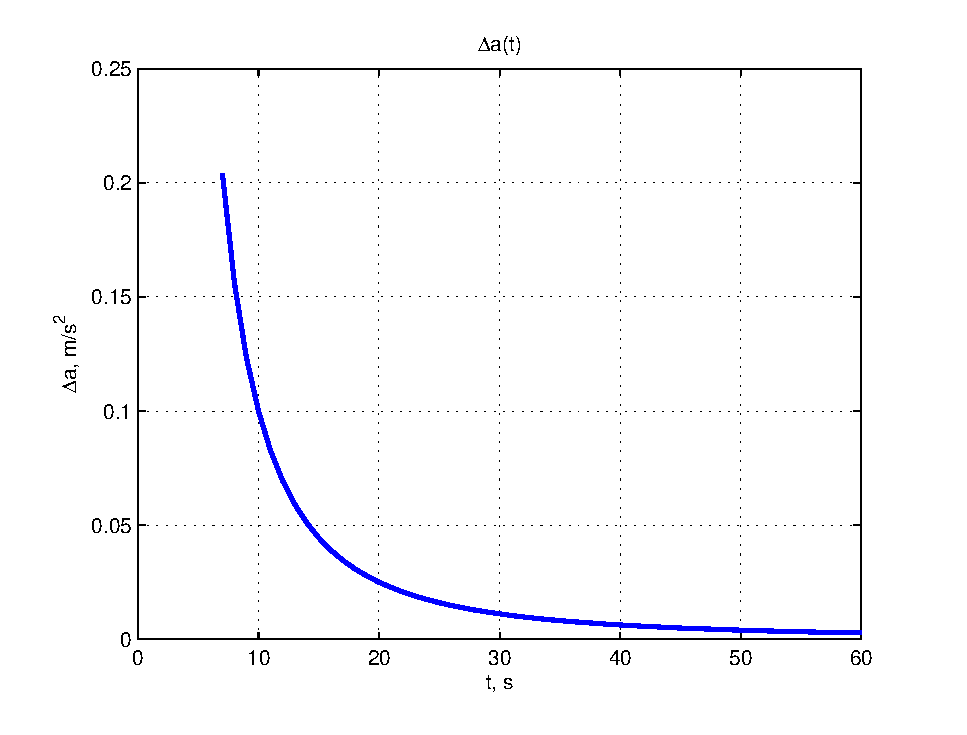
\includegraphics[scale=0.8]{acc_err}
\caption{Графік залежності значень похибок акселерометра від часу}
\label{fig:acc_err}
\end{figure} 
\vline 

\textit{Оцінка помилки датчика кутової швидкості}

Якщо вимірник кутової швидкості об'єкта має погрішність $\Delta \vartheta '$, то приладове значення кутової швидкості

\[\dot{\vartheta }'^{*} =\dot{\vartheta }'-\Delta \dot{\vartheta }'.\] 

При цьому, будуть мати місце помилки у визначенні інших параметрів.

Підставляючи значення параметрів $\dot{\vartheta }'^{*} $ і  $\lambda _{y}^{*} $ рівняння \eqref{eq:ddot_lambda_1},  після перетворень з врахуванням другого рівняння системи \eqref{eq:err} одержимо

\begin{equation} 
\label{eq:err_lambda_dot} 
\Delta \ddot{\lambda }_{y} +\frac{a_{\eta } +g_{0} }{R_{\text{З}} } \Delta \lambda _{y} =-\frac{a_{\eta } +g_{0} }{R_{\text{З}} } \Delta \vartheta ' 
\end{equation} 

Як видно ліва частина рівняння \eqref{eq:err_lambda_dot} і в цьому випадку (при $a_{\eta } =0$) представляється рівняння маятника Шулера, а права частина -- фактор, що викликається, обумовленими погрішностями у вимірі $\vartheta '$кута .

Якщо вважати погрішність $\Delta \dot{\vartheta }'=\Delta \dot{\vartheta }'_{0} =const$, то $\Delta \vartheta '=\Delta \dot{\vartheta }'_{0} t$, при цьому рішення рівняння 
\eqref{eq:err_lambda_dot} буде (якщо $a_{\eta } =0$) наступної:

\begin{equation} 
\label{eq:err_lambda_delta} 
\Delta \lambda _{y} =\Delta \dot{\vartheta }'_{0} \left(\sqrt{\frac{R_{\text{З}} }{g_{0} } } \sin \sqrt{\frac{g_{0} }{R_{\text{З}} } } \cdot t-t\right)
\end{equation} 


Як видно з виразу \eqref{eq:err_lambda_delta},  погрішність у визначенні координати  $\lambda _{y} $, обумовлена постійною  помилкою  вимірника кутової швидкості, у першому наближенні має дві складові (рис. 2.5,\textit{б)}, одна  з яких  росте пропорційно  часу польоту

\[\Delta \lambda _{y0} =\Delta \dot{\vartheta }'_{0} t,\] 

а інша  змінюється з періодом маятника Шулера

\[\Delta \lambda _{y} =\Delta \dot{\vartheta }'_{0} \sqrt{\frac{R_{\text{З}} }{g_{0} } } \sin \sqrt{\frac{g_{0} }{R_{\text{З}} } } \cdot t\] 


Аналогічно \eqref{eq:acc_err} можуть бути отримані орієнтовані формули для розрахунку точносних вимог 
пропонованих до вимірників кутових швидкостей.

\[\Delta \dot{\vartheta }'_{0} =\frac{\Delta \lambda _{y} }{\left(\sqrt{\frac{R_{{\text{З}}} }{g_{0} } } \sin \left(\sqrt{\frac{g_{0} }{R_{{\text{З}}} } } \cdot t\right)-t\right)} \] 

Виходячи з вимог пропонованих до точносних характеристик визначення координат (СКО $\approx$ 5м) 
отримані орієнтовані значення похибок вимірникам кутових швидкостей, у залежності від очікуваних 
перерв у роботі супутникової системи навігації. Розрахункові значення точнісних вимоги пропонованих 
до датчиків первинної інформації, зокрема вимірникам кутових швидкостей відображені на графіку рис.\ref{fig:gyro_err}.

\begin{figure}[here]
\centering
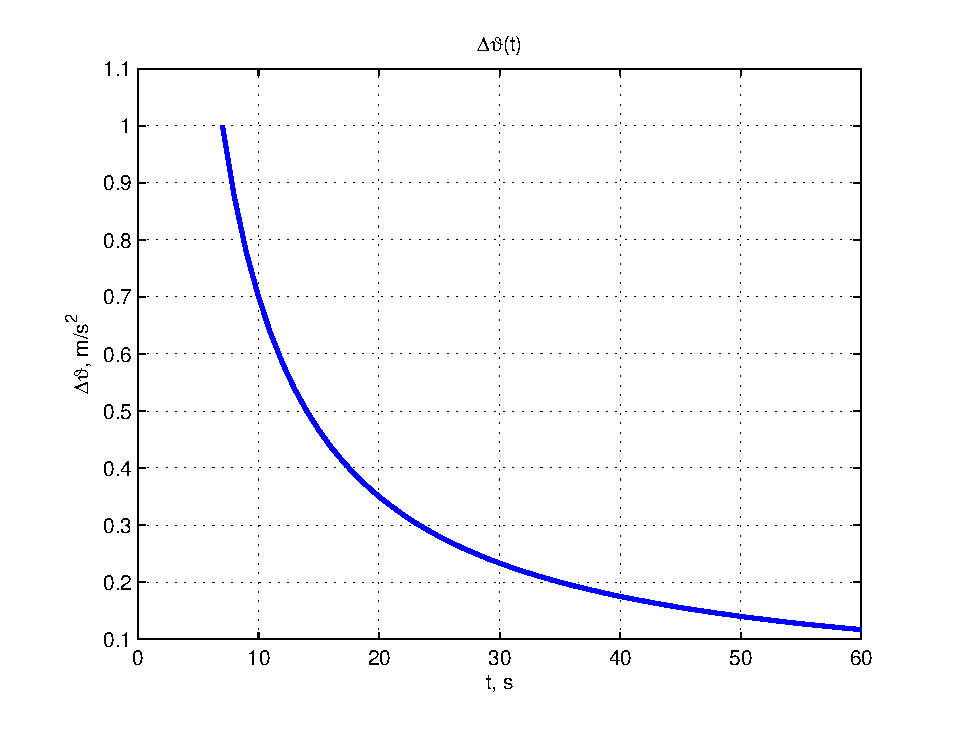
\includegraphics[scale=0.8]{gyro_err}
\caption{Графік залежності значень похибок ДКШ від часу}
\label{fig:gyro_err}
\end{figure} 

Для БІНС розглянутого класу основний внесок у похибки визначення координат вносять датчики первинної 
інформації. Необхідно відзначити, що методичні похибки, у тому числі похибки, зв'язані зі спрощеннями 
кінематичних рівнянь БІНС, похибками моделювання форми Землі і похибками моделі гравітаційного поля, 
повинні бути не більше  похибок, внесених датчиками первинної інформації.

Багато складові вихідні похибки залежать від параметрів траєкторії й умов роботи, коефіцієнти моделі 
похибок істотно залежать від рівня вібрації і температури. Тому для більш детального дослідження 
точністних характеристик  БІНС необхідна вихідна інформація про аеродинамічні й інерційно масові 
характеристиках літака, а також параметри траєкторії. У цьому випадку можна буде провести детальні 
статистичні дослідження точністних характеристик з урахуванням впливу динамічних похибок датчиків первинної інформації.

Однак при моделюванні враховувалися тільки деякі складові:
\begin{enumerate}
  \item систематичні;
%  \item перекручування масштабного коефіцієнта;
  \item випадкові складові;
%  \item зони нечутливості
\end{enumerate}

Випадкові складові і перекручування масштабного коефіцієнта моделювалися 
з використанням генераторів "білого шуму" і формуючих фільтрів. При цьому 
вважалося, що кожен чуттєвий елемент цілком визначається значеннями цих 
складових, а самі ці складові змінюються таким чином, що при збільшенні 
одного з них зростають і всі інші. 

\begin{figure}[here]
\centering
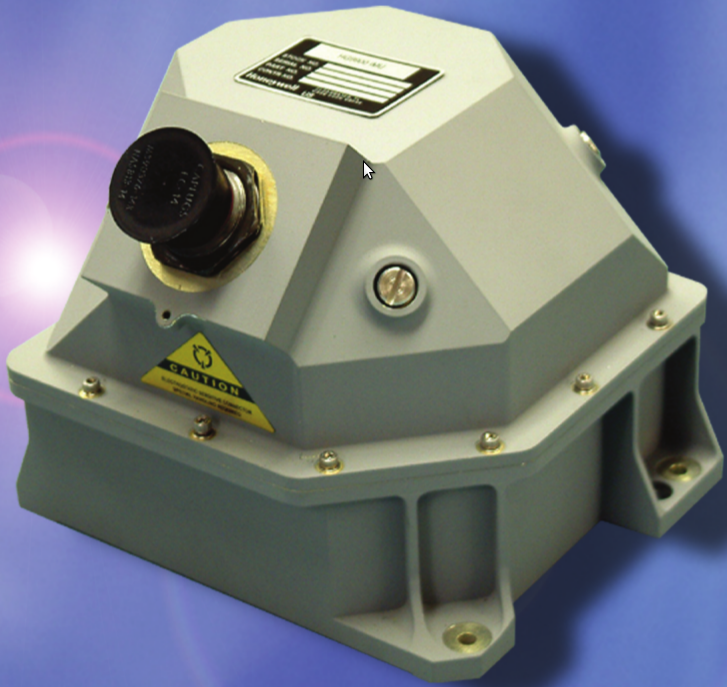
\includegraphics[scale=0.3]{imu_hg9900}
\caption{ДПІ Honeywell HG9900IMU}
\label{fig:imu_hg9900}
\end{figure} 

В роботі пропонується датчики первинної інформації \textit{HG9900IMU} (рис.\ref{fig:imu_hg9900}),
які базуються на лазерних гіроскопах \textit{Honeywell GG1320AN01} та кварцових акселерометрах \textit{Honeywell QA-2000}. Всі датчики знаходяться в протиударному герметичному корпусі. Параметри ДПІ показані в таблицях \ref{tab:gyro_params},\ref{tab:acc_params}.
\nomenclature{IMU}{Inertial Measurement Unit}

\begin{table}[H]
\centering
\caption{Параметри IMU HG9900}

\begin{tabular}{|p{60mm}|p{70mm}|} \hline

Процесор & TI DSP TMS320VC33 (60 Mips) \\ \hline 
Пам’ять & 128 Kbytes SRAM, 512 Kbytes Flash EEPROM \\ \hline 
Ввід/вивід & SDLC RS-422 \\ \hline 
Частота & 300 Hz  \\ \hline 
Живлення & 5, $\pm$15 Vdc input \\ \hline 
Потужність& <10W \\ \hline 
Вага & 2.948 кг  \\ \hline 
Температурний діапазон & $-54^{o}$C до $+71^{o}$C  \\ \hline
Розміри & $5.5\times6.4\times5.34 inch$\\ \hline 
\end{tabular}
\label{tab:imu_params}
\end{table}


\begin{table}[H]
\centering
\caption{Параметри гіроскопів GG1320AN01}
\begin{tabular}{|p{70mm}|p{40mm}|} \hline
Дрейф & <0.003 deg/hr \\ \hline 
Випадкове блукання &<0.002 deg/$\sqrt{hr}$  \\ \hline 
Коефіцієнт масштабування & <5.0 PPM  \\ \hline 
\end{tabular}
\label{tab:gyro_params}
\end{table}

\begin{table}[H]
\centering
\caption{Параметри акселерометрів QA-2000}
\begin{tabular}{|p{70mm}|p{40mm}|} \hline
Дрейф & <25 $\mu g$ \\ \hline 
Випадкове блукання &<0.002 deg/$\sqrt{hr}$  \\ \hline 
Коефіцієнт масштабування & <100 PPM  \\ \hline 
\end{tabular}
\label{tab:acc_params}
\end{table}

Іншою перевагою вказаних датчиків є присутність, температурних сенсорів, що за допомогою спеціально створеного алгоритму, компенсує температурний дрейф параметрів (наприклад масштабний коефіцієнт, не ортогональність осей). 